\documentclass[11pt]{article}
\usepackage[margin=1in]{geometry}
\usepackage{lmodern}
\usepackage[T1]{fontenc}
\usepackage{microtype}
\usepackage{amsmath,amssymb,mathtools,bm}
\usepackage{booktabs,array,tabularx}
\usepackage{graphicx}
\usepackage{caption,subcaption}
\usepackage{enumitem}
\usepackage[section]{placeins}   % floats stay in their section
\usepackage{xcolor}
\usepackage{tikz}
\usetikzlibrary{arrows.meta,calc,decorations.markings,patterns}
\usepackage{algorithm}
\usepackage{algpseudocode}
\usepackage[hyphens]{url}
\usepackage[colorlinks=true,linkcolor=blue!50!black,urlcolor=blue!60!black,citecolor=blue!50!black]{hyperref}

\sloppy
\emergencystretch=3em

% \code{...}: \texttt that may break after an underscore
\makeatletter
\newcommand{\code}[1]{{\def\_{\char`\_\discretionary{}{}{}}\texttt{#1}}}
\makeatother

% Permalinks into the Jexpresso source at the commit this document describes.
\newcommand{\jxrepo}{https://github.com/smarras79/Jexpresso/blob/2ab96bf169f1eb9e5702936f4ef7b55b710ddc3d}
\newcommand{\jx}[3]{\href{\jxrepo/#1\#L#2}{\code{#3}}}
\newcommand{\jxfile}[2]{\href{\jxrepo/#1}{\code{#2}}}
\newcommand{\coderef}[1]{\par\smallskip\noindent{\small\textcolor{black!65}{\textsf{Code:}}~#1}\par\smallskip}

\newcommand{\dev}{\operatorname{dev}}
\newcommand{\tr}{\operatorname{tr}}
\newcommand{\sym}{\operatorname{sym}}
\newcommand{\bu}{\bm{u}}
\newcommand{\bv}{\bm{v}}
\newcommand{\bx}{\bm{x}}
\newcommand{\bn}{\bm{n}}
\newcommand{\bsig}{\bm{\sigma}}
\newcommand{\beps}{\bm{\varepsilon}}
\newcommand{\be}{\bm{e}}
\newcommand{\bq}{\bm{q}}
\newcommand{\bs}{\bm{s}}
\newcommand{\bI}{\bm{1}}
\newcommand{\dd}{\,\mathrm{d}}

\title{Quasi-static viscoelastic and elasto-plastic solids\\ on Jexpresso's spectral elements\\[4pt]
\large The thick-walled cylinder and the perforated plate of\\ Artioli, Beir\~ao da Veiga, Lovadina \& Sacco (2017), \S\S4.2--4.3}
\author{Jexpresso, branch \texttt{sm/solid}, commit \href{https://github.com/smarras79/Jexpresso/commit/2ab96bf169f1eb9e5702936f4ef7b55b710ddc3d}{\texttt{2ab96bf}}}
\date{}

\begin{document}
\maketitle

\begin{abstract}
This note documents the quasi-static solid-mechanics path of Jexpresso
(\code{:lquasistatic\_solid}) and the benchmark it was built for: a plane-strain
thick-walled cylinder under a step internal pressure, made of a generalized
Maxwell viscoelastic material (Artioli et al.\ 2017, Secs.~3.1 and~4.2). It
states the governing equations, the constitutive laws (the viscoelastic one of
the benchmark and the $J_2$ plasticity that uses the same quadrature-point
history), every step of the spectral-element discretisation, and the
initialisation, and links each to the line of the Jexpresso source where it is
done. Section~\ref{sec:plate} adds the paper's second inelastic benchmark, a
perforated elastic--perfectly plastic plate (\S4.3), and the script that redraws
the paper's figures from Jexpresso's VTK output. Every link is a permalink to
commit \texttt{2ab96bf}.
\end{abstract}

\tableofcontents

%==============================================================================
\section{The problem}\label{sec:setup}
%==============================================================================

A long cylinder of inner radius $a=2$ and outer radius $b=4$ is loaded by an
internal pressure $p=10$ switched on at $t=0$ and held to $t=20$; the outer
surface is free. The cylinder is long, so the state is \emph{plane strain}
($u_z=0$, $\varepsilon_{zz}=0$), and by symmetry one quarter of the
cross-section is modelled, with rollers on the two straight edges
(Fig.~\ref{fig:setup}). The control points are $A=(a,0)$ on the bore and
$B=(b,0)$ on the outer surface, where $u_r=u_x$.

\begin{figure}[ht]
\centering
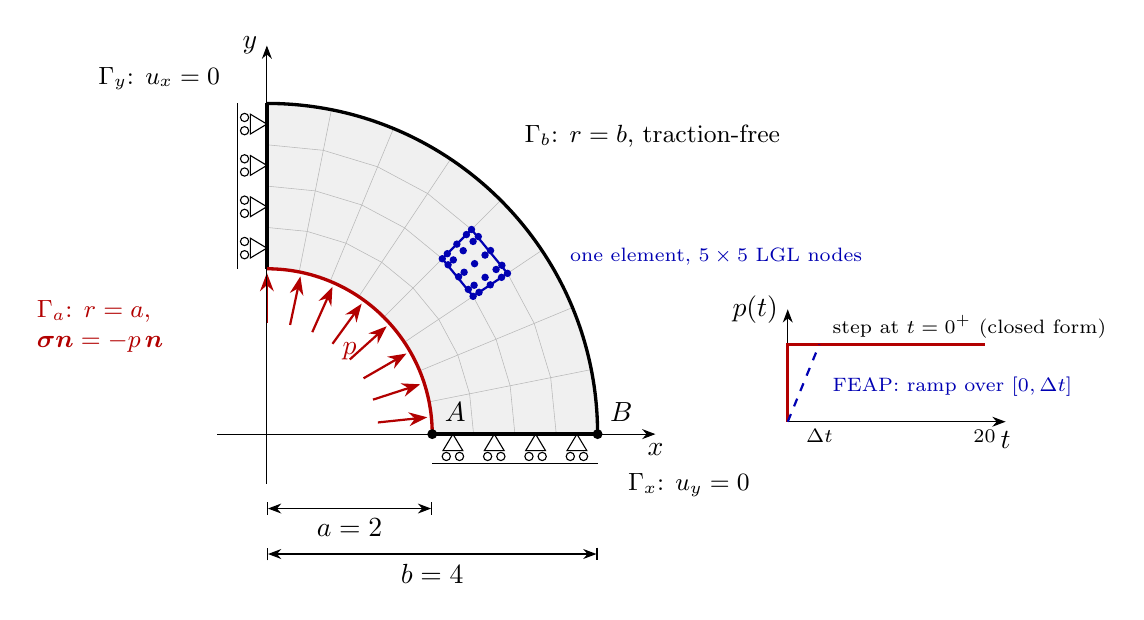
\begin{tikzpicture}[scale=1.05,>=Stealth]
  \def\a{2.0}\def\b{4.0}
  % body
  \fill[gray!12] (\a,0) -- (\b,0) arc[start angle=0,end angle=90,radius=\b] -- (0,\a) arc[start angle=90,end angle=0,radius=\a] -- cycle;
  % SEM grid: 4 radial x 8 circumferential elements (interior edges are chords)
  \foreach \k in {1,...,7}{ \draw[gray!55,very thin] ({\a*cos(11.25*\k)},{\a*sin(11.25*\k)}) -- ({\b*cos(11.25*\k)},{\b*sin(11.25*\k)}); }
  \foreach \r in {2.5,3.0,3.5}{ \draw[gray!55,very thin] plot[domain=0:8,samples=9] ({\r*cos(11.25*\x)},{\r*sin(11.25*\x)}); }
  % one element (r in [3, 3.5], theta in [33.75, 45] deg) with its 5x5 LGL nodes (N = 4)
  \draw[blue!70!black,thick] ({3.0*cos(33.75)},{3.0*sin(33.75)}) -- ({3.5*cos(33.75)},{3.5*sin(33.75)})
        -- ({3.5*cos(45)},{3.5*sin(45)}) -- ({3.0*cos(45)},{3.0*sin(45)}) -- cycle;
  \foreach \xi in {-1,-0.6547,0,0.6547,1}{\foreach \eta in {-1,-0.6547,0,0.6547,1}{
      \pgfmathsetmacro{\rr}{3.25+0.25*\xi}\pgfmathsetmacro{\tt}{39.375+5.625*\eta}
      \fill[blue!70!black] ({\rr*cos(\tt)},{\rr*sin(\tt)}) circle (0.045);}}
  \node[blue!70!black,font=\scriptsize,anchor=west] at (3.55,2.15) {one element, $5\times5$ LGL nodes};
  % boundaries
  \draw[very thick] (\a,0) -- (\b,0);
  \draw[very thick] (0,\a) -- (0,\b);
  \draw[very thick,red!70!black] (\a,0) arc[start angle=0,end angle=90,radius=\a];
  \draw[very thick] (\b,0) arc[start angle=0,end angle=90,radius=\b];
  % pressure arrows on the bore (pointing into the wall)
  \foreach \t in {6,18,...,90}{ \draw[->,red!70!black,thick] ({1.35*cos(\t)},{1.35*sin(\t)}) -- ({1.95*cos(\t)},{1.95*sin(\t)}); }
  \node[red!70!black] at (1.0,1.0) {$p$};
  % rollers on y = 0 (u_y = 0)
  \foreach \x in {2.25,2.75,...,3.75}{ \draw (\x,0) -- (\x-0.12,-0.2) -- (\x+0.12,-0.2) -- cycle; \draw (\x-0.08,-0.27) circle (0.05); \draw (\x+0.08,-0.27) circle (0.05);}
  \draw (2.0,-0.35) -- (4.0,-0.35);
  % rollers on x = 0 (u_x = 0)
  \foreach \y in {2.25,2.75,...,3.75}{ \draw (0,\y) -- (-0.2,\y-0.12) -- (-0.2,\y+0.12) -- cycle; \draw (-0.27,\y-0.08) circle (0.05); \draw (-0.27,\y+0.08) circle (0.05);}
  \draw (-0.35,2.0) -- (-0.35,4.0);
  % axes
  \draw[->] (-0.6,0) -- (4.7,0) node[below] {$x$};
  \draw[->] (0,-0.6) -- (0,4.7) node[left] {$y$};
  % points
  \fill (\a,0) circle (0.06) node[above right=1pt] {$A$};
  \fill (\b,0) circle (0.06) node[above right=1pt] {$B$};
  % radii
  \draw[|<->|,thin] (0,-0.9) -- node[below] {$a=2$} (\a,-0.9);
  \draw[|<->|,thin] (0,-1.45) -- node[below] {$b=4$} (\b,-1.45);
  % labels
  \node[align=left,anchor=west,font=\small] at (3.0,3.6) {$\Gamma_b$: $r=b$, traction-free};
  \node[align=left,anchor=west,font=\small,red!70!black] at (-2.9,1.3) {$\Gamma_a$: $r=a$,\\ $\bsig\bn=-p\,\bn$};
  \node[align=left,anchor=west,font=\small] at (4.25,-0.62) {$\Gamma_x$: $u_y=0$};
  \node[align=left,anchor=east,font=\small] at (-0.45,4.3) {$\Gamma_y$: $u_x=0$};
  % load history inset
  \begin{scope}[shift={(6.3,0.15)},scale=0.85]
    \draw[->] (0,0) -- (3.1,0) node[below] {$t$};
    \draw[->] (0,0) -- (0,1.6) node[left] {$p(t)$};
    \draw[very thick,red!70!black] (0,0) -- (0,1.1) -- (2.8,1.1);
    \draw[thick,dashed,blue!70!black] (0,0) -- (0.45,1.1);
    \node[font=\scriptsize,anchor=west] at (0.5,1.35) {step at $t=0^+$ (closed form)};
    \node[font=\scriptsize,anchor=west,blue!70!black] at (0.5,0.5) {FEAP: ramp over $[0,\Delta t]$};
    \node[font=\scriptsize] at (0.45,-0.2) {$\Delta t$};
    \node[font=\scriptsize] at (2.8,-0.2) {$20$};
  \end{scope}
\end{tikzpicture}
\caption{The quarter cylinder (plane strain) and its boundary conditions, drawn over
the spectral-element grid of the case: $4\times8$ quadrilaterals, both arcs curved
onto their circles; one element shows its $5\times5$ LGL nodes ($N=4$). Inset: the
pressure history --- the Heaviside step of the closed form, and the ramp over the
first increment that the paper's FEAP runs amount to (\S\ref{sec:init}).}
\label{fig:setup}
\end{figure}

\begin{table}[ht]
\centering
\small
\begin{tabularx}{\textwidth}{@{}lXl@{}}
\toprule
quantity & value & note\\
\midrule
Young's modulus, Poisson's ratio & $E=1000$, $\nu=0.3$ & instantaneous\\
shear, bulk modulus & $G=E/2(1+\nu)=384.6$, $K=E/3(1-2\nu)=833.3$ & \\
Prony series & $G(t)=G\,(\mu_0+\mu_1e^{-t/\lambda})$, $\lambda=1$ & $\lambda$: relaxation time\\
set ve1 / ve2 & $(\mu_0,\mu_1)=(0.01,0.99)$ / $(0.3,0.7)$ & \code{JEXPRESSO\_VE\_SET}\\
geometry, load & $a=2$, $b=4$, $p=10$, $t\in[0,20]$ & \\
discretisation & $N=4$, $4\times8$ elements, $\Delta t=1$ & 1122 DOFs\\
\bottomrule
\end{tabularx}
\caption{Data of the benchmark. Note: the paper's $\lambda$ is a \emph{relaxation time};
it has nothing to do with the Lam\'e constant, which is why the code calls it $\tau$.}
\label{tab:data}
\end{table}

\coderef{the case: \jxfile{problems/Elasticity/viscoelastic_cylinder2d}{problems/Elasticity/viscoelastic\_cylinder2d};
deck \jx{problems/Elasticity/viscoelastic_cylinder2d/user_inputs.jl}{26}{user\_inputs};
material, geometry, load \jx{problems/Elasticity/viscoelastic_cylinder2d/user_flux.jl}{41}{cylinder\_properties};
mesh \jx{problems/Elasticity/make_meshes.py}{74}{structured\_quarter\_annulus}.}

%==============================================================================
\section{Governing equations}\label{sec:equations}
%==============================================================================

Small strains, no inertia (the loading is slow compared with the elastic wave
transit, so the problem is \emph{quasi-static}), no body force. For every
$t\in[0,T]$ find the displacement $\bu(\bx,t)$ on the quarter cross-section
$\Omega$ such that
\begin{align}
  \nabla\!\cdot\bsig + \bm b &= \bm 0 && \text{in } \Omega, \label{eq:equilibrium}\\
  \beps(\bu) &= \sym\nabla\bu = \tfrac12(\nabla\bu+\nabla\bu^{\mathsf T}), \quad \varepsilon_{zz}=0
                                           && \text{(plane strain)}, \label{eq:strain}\\
  \bsig\bn &= -p(t)\,\bn && \text{on } \Gamma_a\ (r=a), \label{eq:pressure}\\
  \bsig\bn &= \bm 0      && \text{on } \Gamma_b\ (r=b), \label{eq:free}\\
  u_y &= 0,\ \ (\bsig\bn)_x = 0 && \text{on } \Gamma_x\ (y=0), \label{eq:rollerx}\\
  u_x &= 0,\ \ (\bsig\bn)_y = 0 && \text{on } \Gamma_y\ (x=0), \label{eq:rollery}
\end{align}
with $\bn$ the outward unit normal and $\bsig$ given by the constitutive law of
\S\ref{sec:constitutive}, which carries the memory of the material. Time enters
\emph{only} through that memory and through $p(t)$.

\paragraph{Weak form.} With $V=\{\bv\in H^1(\Omega)^2: v_y=0 \text{ on } \Gamma_x,\ v_x=0 \text{ on } \Gamma_y\}$,
find $\bu(t)\in V$ such that
\begin{equation}
  \int_\Omega \beps(\bv):\bsig\dd\Omega
  = \int_{\Gamma_a} \bv\cdot(-p\,\bn)\dd\Gamma + \int_\Omega \bv\cdot\bm b\dd\Omega
  \qquad \forall\,\bv\in V .
  \label{eq:weak}
\end{equation}
Only the in-plane components of $\bsig$ appear ($\varepsilon_{zz}(\bv)=0$), but
the material point is three-dimensional and $\sigma_{zz}$ is part of the
solution.

\coderef{boundary conditions \jx{problems/Elasticity/viscoelastic_cylinder2d/user_bc.jl}{24}{user\_solid\_bc};
body force \jx{problems/Elasticity/viscoelastic_cylinder2d/user_source.jl}{8}{user\_solid\_body\_force};
the solver and its documentation \jx{src/kernel/solvers/quasistatic_solid.jl}{1}{quasistatic\_solid.jl};
dispatch from the driver \jx{problems/drivers.jl}{262}{drivers.jl}.}

%==============================================================================
\section{Constitutive laws}\label{sec:constitutive}
%==============================================================================

\subsection{Generalized Maxwell viscoelasticity (the benchmark)}

Volumetric--deviatoric split, $\beps=\be+\tfrac13\tr(\beps)\bI$, elastic in volume
and generalized Maxwell in the deviator (Artioli et al.\ eqs.~3.2--3.7):
\begin{equation}
  \bsig = K\,\tr(\beps)\,\bI + \bs,\qquad
  \bs(t)=\int_{-\infty}^{t} 2G(t-s)\,\dot\be(s)\dd s,\qquad
  G(t) = G\Big(\mu_0+\sum_{m=1}^{M}\mu_m e^{-t/\lambda_m}\Big),
  \label{eq:ve}
\end{equation}
with $\mu_0+\sum_m\mu_m=1$. Each Prony term is a spring--dashpot branch whose
spring strain $\bq_m$ (a deviatoric tensor) obeys
\begin{equation}
  \dot\bq_m + \frac{1}{\lambda_m}\bq_m = \dot\be,
  \qquad \bs = 2G\Big(\mu_0\,\be+\sum_m \mu_m\bq_m\Big).
  \label{eq:maxwell}
\end{equation}
In plane strain $e_{zz}=-\tfrac13\tr\beps\neq0$, so $\bq_m$ and $\bs$ have four
non-zero components $(xx,yy,zz,xy)$ and $\sigma_{zz}=K\tr\beps+s_{zz}$ creeps.

\paragraph{Time integration: the exponential recursion.} Integrating
\eqref{eq:maxwell} exactly over $[t_n,t_{n+1}]$ for a strain that is linear in
time (Zienkiewicz, Taylor \& Fox 2014; Simo \& Hughes 1998, \S10.3) gives
\begin{equation}
  \bq_m^{n+1} = d_m\,\bq_m^n + \gamma_m\big(\be^{n+1}-\be^n\big),\qquad
  d_m=e^{-\Delta t/\lambda_m},\quad
  \gamma_m=\frac{\lambda_m}{\Delta t}\big(1-e^{-\Delta t/\lambda_m}\big),
  \label{eq:recursion}
\end{equation}
second-order accurate; it is the update FEAP --- and so the paper --- uses.
Simo \& Hughes' Box~10.1 variant $\gamma_m=e^{-\Delta t/2\lambda_m}$ is also
second order; backward Euler $d_m=\gamma_m=(1+\Delta t/\lambda_m)^{-1}$ is first
order. Because \eqref{eq:recursion} is linear in $\be^{n+1}$,
\begin{equation}
  \bsig^{n+1} = K\tr(\beps^{n+1})\bI + 2\tilde G\,\be^{n+1} + \bsig^{*},\qquad
  \tilde G = G\Big(\mu_0+\sum_m\mu_m\gamma_m\Big),\quad
  \bsig^{*}=2G\sum_m\mu_m\big(d_m\bq_m^n-\gamma_m\be^n\big):
  \label{eq:algorithmic}
\end{equation}
each step is a linear elastic problem with the \emph{algorithmic} shear modulus
$\tilde G$ and a known initial stress $\bsig^*$. For $\Delta t=0$,
$d_m=\gamma_m=1$: the instantaneous (glassy) response.

\coderef{coefficients $(d_m,\gamma_m)$ \jx{src/kernel/solvers/quasistatic_solid.jl}{177}{maxwell\_step\_coefficients};
the material point \jx{src/kernel/solvers/quasistatic_solid.jl}{293}{solid\_constitutive\_update!};
the case's material \jx{problems/Elasticity/viscoelastic_cylinder2d/user_flux.jl}{71}{user\_solid\_material}.}

\paragraph{Closed-form solution.} By the correspondence principle (load $p/s$,
$G\to s\hat G(s)$, $K$ unchanged), for the Heaviside pressure
\begin{gather}
  u_r(r,t) = P\Big[r\,C(t)+\frac{b^2}{2r}J(t)\Big],\qquad P=\frac{p\,a^2}{b^2-a^2},\\
  J(t)=\frac1G\Big[\frac{1}{\mu_0}-\Big(\frac{1}{\mu_0}-1\Big)e^{-\mu_0t/\lambda}\Big]
  \quad\text{(shear creep compliance)},\\
  C(t)=\frac1{M_\infty}-\Big(\frac1{M_\infty}-\frac1{M_0}\Big)e^{-M_\infty t/(M_0\lambda)},\qquad
  M_0=2K+\tfrac23G,\quad M_\infty=2K+\tfrac23\mu_0G .
\end{gather}
At $t=0$ it is the Lam\'e solution $P\,\frac{1+\nu}{E}\big[(1-2\nu)r+b^2/r\big]$.
$\sigma_{rr}=P(1-b^2/r^2)$ and $\sigma_{\theta\theta}=P(1+b^2/r^2)$ do not depend on
the material (both surfaces carry tractions), so they are the Lam\'e stresses at
every $t$; what creeps is $u_r$ and
$\sigma_{zz}(t)=2P\big[\nu_\infty+(\nu-\nu_\infty)e^{-t/\tau_z}\big]$, with
$\nu_\infty=\frac{3K-2\mu_0G}{2(3K+\mu_0G)}$, $\tau_z=\lambda\frac{3K+G}{3K+\mu_0G}$.
\coderef{\jx{problems/Elasticity/viscoelastic_cylinder2d/user_analytic.jl}{69}{cylinder\_ur\_exact},
\jx{problems/Elasticity/viscoelastic_cylinder2d/user_analytic.jl}{76}{cylinder\_szz\_exact},
and the exact-in-space time-discrete reference
\jx{problems/Elasticity/viscoelastic_cylinder2d/user_analytic.jl}{129}{cylinder\_time\_discrete\_reference}.}

\subsection{$J_2$ plasticity: the history at the quadrature points}

The same path carries models whose history is \emph{not} a linear function of
the displacement, and stores it at every quadrature point. Von Mises
plasticity with linear isotropic and kinematic hardening (Artioli et al.\
\S3.2; Simo \& Hughes Box~3.2):
\begin{gather}
  \bs = 2G(\be-\be^p),\quad \bm\alpha = H_{\mathrm{kin}}\,\be^p,\quad \bm X=\bs-\bm\alpha,\quad
  f = \|\bm X\| - \sqrt{\tfrac23}\big(\sigma_{y0}+H_{\mathrm{iso}}\,\bar e^p\big)\le0,\\
  \dot\be^p = \dot\zeta\,\frac{\bm X}{\|\bm X\|},\qquad
  \dot{\bar e}^p=\sqrt{\tfrac23}\,\dot\zeta,\qquad \dot\zeta\ge0,\ \dot\zeta f=0 .
\end{gather}
History per point: $\be^p$ (four components) and $\bar e^p$. Backward Euler
gives the radial return: trial $\bm X^{\mathrm{tr}}=2G(\be^{n+1}-\be^{p,n})-H_{\mathrm{kin}}\be^{p,n}$;
if $f^{\mathrm{tr}}>0$, $\Delta\zeta=f^{\mathrm{tr}}/(2G+H_{\mathrm{kin}}+\tfrac23H_{\mathrm{iso}})$,
$\bm n=\bm X^{\mathrm{tr}}/\|\bm X^{\mathrm{tr}}\|$, $\be^{p,n+1}=\be^{p,n}+\Delta\zeta\bm n$,
and the consistent tangent is
\begin{equation}
  \mathbb C = K\,\bI\otimes\bI + 2G\theta\,\mathbb I_{\dev} - 2G\bar\theta\,\bm n\otimes\bm n,\quad
  \theta = 1-\frac{2G\Delta\zeta}{\|\bm X^{\mathrm{tr}}\|},\quad
  \bar\theta=\frac{2G}{2G+H_{\mathrm{kin}}+\frac23H_{\mathrm{iso}}}-(1-\theta).
\end{equation}
A shape-memory alloy (Artioli et al.\ \S3.3) keeps the transformation strain
$\be^{tr}$ where $J_2$ keeps $\be^p$: the storage, the Newton loop of
Step~7 (\S\ref{sec:sem}) and the output are the same.
\coderef{\jx{src/kernel/solvers/quasistatic_solid.jl}{317}{solid\_constitutive\_update!} ($J_2$);
history layout and plottable fields \jx{src/kernel/solvers/quasistatic_solid.jl}{218}{solid\_history\_fields};
the plasticity case \jxfile{problems/Elasticity/plastic_cylinder2d}{problems/Elasticity/plastic\_cylinder2d}.}

%==============================================================================
\section{Spectral-element discretisation, step by step}\label{sec:sem}
%==============================================================================

Every spatial operator below is Jexpresso's own; the solver adds the material
and the time stepping.

\subsection*{Step 1 --- the grid}
gmsh writes a structured, \emph{straight-sided} grid of $4\times8$ quadrilaterals
with the physical groups \code{inner}, \code{outer}, \code{xaxis}, \code{yaxis}
and \code{domain}. Jexpresso reads it, places on each element the
$(N+1)^2$ Legendre--Gauss--Lobatto (LGL) nodes $\bm\xi_{ij}=(\xi_i,\xi_j)$ of
degree $N=4$, and numbers the nodes globally through the connectivity
$\mathrm{conn}(e,i,j)$ (\code{connijk}). gmsh leaves every high-order node of
an arc on its chord; \code{:exact\_geometry} snaps the boundary nodes onto the
circles $r=a$ and $r=b$ and blends the correction into the boundary elements
(Gordon--Hall), so the boundary is the isoparametric degree-$N$ interpolant of
the circle.
\coderef{\jx{problems/Elasticity/make_meshes.py}{74}{make\_meshes.py};
\jx{src/kernel/mesh/mesh.jl}{1744}{mod\_mesh\_read\_gmsh!};
\jx{src/kernel/mesh/exact_geometry.jl}{1}{exact\_geometry.jl} (called at
\jx{src/kernel/mesh/mesh.jl}{3829}{mesh.jl});
deck \jx{problems/Elasticity/viscoelastic_cylinder2d/user_inputs.jl}{91}{:exact\_geometry}.}

\subsection*{Step 2 --- basis, quadrature and metric terms}
On the reference square the basis is the tensor product of the degree-$N$
Lagrange polynomials through the LGL nodes,
$\psi_{ij}(\xi,\eta)=\ell_i(\xi)\ell_j(\eta)$, and the displacement is
\begin{equation}
  \bu_h(\bx)=\sum_{a}\psi_a(\bx)\,\bu_a,\qquad a=\mathrm{conn}(e,i,j).
\end{equation}
Integrals use the LGL rule on the same nodes (collocation, $Q=N$; Jexpresso's
\code{Inexact} quadrature), weights $\omega_k\omega_l$. The map
$\bx(\xi,\eta)=\sum\psi_{ij}\bx_{ij}$ gives the metric terms
$\partial\xi/\partial x,\dots$ and $J$ at every node; with them
\begin{equation}
  \frac{\partial\psi_{ij}}{\partial x}\Big|_{kl}=\ell_i'(\xi_k)\ell_j(\xi_l)\,\xi_x+\ell_i(\xi_k)\ell_j'(\xi_l)\,\eta_x,
  \qquad
  \int_{\Omega_e} g\dd\Omega\approx\sum_{k,l}\omega_k\omega_l\,J_{kl}\,g_{kl}.
\end{equation}
On a boundary edge, the surface Jacobian $J^f=|\mathrm d\bx/\mathrm d\xi|$ and the
outward normal come from the tangent of the same degree-$N$ interpolant, so they
are right on the curved arcs.
\coderef{\jx{src/kernel/infrastructure/sem_setup.jl}{132}{sem\_setup};
\jx{src/kernel/mesh/metric_terms.jl}{197}{build\_metric\_terms!} (2D, with the boundary normals and $J^f$ at
\jx{src/kernel/mesh/metric_terms.jl}{260}{metric\_terms.jl}).}

\subsection*{Step 3 --- element matrices and direct stiffness summation}
Inserting $\bu_h$ and $\bv=\psi_a\bm e_\alpha$ into \eqref{eq:weak} with the
Voigt form $\bsig=\mathbf D\,\beps$ ($\beps=(\varepsilon_{xx},\varepsilon_{yy},\gamma_{xy})$,
$\gamma_{xy}=2\varepsilon_{xy}$, $\mathbf B_a=[\partial_x\psi_a\ 0;\ 0\ \partial_y\psi_a;\ \partial_y\psi_a\ \partial_x\psi_a]$)
gives the stiffness $\mathbf K_{ab}=\sum_e\int_{\Omega_e}\mathbf B_a^{\mathsf T}\mathbf D\,\mathbf B_b\dd\Omega$.
Jexpresso builds it from the directional element matrices
\begin{equation}
  L^{\alpha\beta}_e[a,b] = \int_{\Omega_e}\partial_\alpha\psi_a\,\partial_\beta\psi_b\dd\Omega
  \approx\sum_{k,l}\omega_k\omega_l J_{kl}\,\partial_\alpha\psi_a\partial_\beta\psi_b\big|_{kl},
\end{equation}
the components of Jexpresso's Laplacian element matrix ($L^{xx}_e+L^{yy}_e$ is
exactly it), assembled by direct stiffness summation (DSS) into sparse global matrices
$S_{\alpha\beta}=\mathrm{DSS}(L^{\alpha\beta})$. For the isotropic material,
$\mathbf D=K\mathbf D_{\mathrm{vol}}+\tilde G\mathbf D_{\mathrm{dev}}$ with
$\mathbf D_{\mathrm{vol}}=\left[\begin{smallmatrix}1&1&0\\1&1&0\\0&0&0\end{smallmatrix}\right]$,
$\mathbf D_{\mathrm{dev}}=\left[\begin{smallmatrix}4/3&-2/3&0\\-2/3&4/3&0\\0&0&1\end{smallmatrix}\right]$,
so in the flat layout $\mathbf u=[\mathbf u_x;\mathbf u_y]$
\begin{equation}
  \mathbf K(\tilde G)=K\,\mathbf A_{\mathrm{vol}}+\tilde G\,\mathbf A_{\mathrm{dev}},\quad
  \mathbf A_{\mathrm{vol}}=\begin{bmatrix}S_{xx}&S_{xy}\\S_{yx}&S_{yy}\end{bmatrix},\quad
  \mathbf A_{\mathrm{dev}}=\begin{bmatrix}\tfrac43S_{xx}+S_{yy}&S_{yx}-\tfrac23S_{xy}\\S_{xy}-\tfrac23S_{yx}&S_{xx}+\tfrac43S_{yy}\end{bmatrix},
  \label{eq:operators}
\end{equation}
$S_{yx}=S_{xy}^{\mathsf T}$, assembled once. When the tangent varies from point
to point (plasticity) the four displacement blocks are built with
$\mathbf D_{kl}$ inside the quadrature sum and assembled the same way.
With LGL collocation the quadrature points are the nodes, so
$\nabla\psi_a$ vanishes at the point $(k,l)$ unless node $a$ shares its row or
its column: $2N+1$ of the $(N+1)^2$ basis functions. Both element routines loop
over those pairs only --- $(2N+1)^2=81$ products per point at $N=4$ instead of
$(N+1)^4=625$ --- accumulating each element in a dense buffer that is scattered
once into the element-matrix layout \code{DSS\_laplace\_sparse} reads.
\coderef{\jx{src/kernel/infrastructure/element_matrices.jl}{375}{build\_laplace\_matrix} and its components
\jx{src/kernel/infrastructure/element_matrices.jl}{453}{build\_gradient\_product\_matrices};
variable tangent \jx{src/kernel/infrastructure/element_matrices.jl}{511}{build\_tangent\_stiffness\_matrices};
the non-zero gradients \jx{src/kernel/infrastructure/element_matrices.jl}{435}{\_element\_basis\_gradients!};
DSS \jx{src/kernel/infrastructure/element_matrices.jl}{839}{DSS\_laplace\_sparse};
assembly of \eqref{eq:operators} \jx{src/kernel/solvers/quasistatic_solid.jl}{379}{solid\_sem\_operators},
\jx{src/kernel/solvers/quasistatic_solid.jl}{404}{solid\_tangent\_matrix}.}

\subsection*{Step 4 --- the load vector}
The pressure \eqref{eq:pressure} is integrated on every boundary edge of
$\Gamma_a$ with the LGL rule of the edge and the curved-edge Jacobian, then
summed onto the nodes:
\begin{equation}
  \mathbf f_a = \sum_{\text{edges}}\sum_{k}\omega_k\,J^f_k\,\big(-p\,\bn_k\big)\,\delta_{a,\mathrm{node}(k)} .
\end{equation}
A body force would enter through the lumped (diagonal) LGL mass matrix,
$\mathbf f_a\mathrel{+}=M_a\bm b(\bx_a)$.
\coderef{\jx{src/kernel/solvers/quasistatic_solid.jl}{545}{solid\_boundary\_conditions!} with Jexpresso's
\jx{src/kernel/boundaryconditions/surface_integral.jl}{45}{compute\_segment\_integral!} and
\jx{src/kernel/boundaryconditions/surface_integral.jl}{54}{DSS\_segment\_integral!};
body force \jx{src/kernel/solvers/quasistatic_solid.jl}{594}{solid\_add\_body\_force!}.}

\subsection*{Step 5 --- the symmetry conditions}
Each roller fixes one Cartesian component ($u_y=0$ on $\Gamma_x$, $u_x=0$ on
$\Gamma_y$); together they remove both translations and the rotation. The
constrained DOFs $c$ are eliminated and the solve is on the free block $f$,
which stays symmetric positive definite:
\begin{equation}
  \mathbf K_{ff}\,\mathbf u_f = \mathbf f_f - \mathbf K_{fc}\,\bar{\mathbf u}_c,\qquad \mathbf u_c=\bar{\mathbf u}_c .
\end{equation}
$\mathbf K_{ff}$ depends on $\Delta t$ only through $\tilde G$, so one sparse
Cholesky factorisation serves every step (a second one the instantaneous step).

\subsection*{Step 6 --- marching in time: the history as a nodal field}
The discrete strain is linear in the nodal displacements and
\eqref{eq:recursion} is linear and starts from zero, so at every quadrature
point $\bq_m=\dev\beps(\mathbf w_m)$ of a \emph{nodal} field $\mathbf w_m$ obeying
the same recursion. With $\mathbf v\cdot\mathbf A_{\mathrm{dev}}\mathbf z=\int\beps(\mathbf v):2\dev\beps(\mathbf z)$,
\eqref{eq:algorithmic} becomes, for every step $n\to n+1$,
\begin{gather}
  \big(K\mathbf A_{\mathrm{vol}}+\tilde G\mathbf A_{\mathrm{dev}}\big)\mathbf u^{n+1}
  = \mathbf f(t_{n+1}) - G\,\mathbf A_{\mathrm{dev}}\sum_m\mu_m\big(d_m\mathbf w_m^n-\gamma_m\mathbf u^n\big),
  \label{eq:nodalstep}\\
  \mathbf w_m^{n+1}=d_m\mathbf w_m^n+\gamma_m(\mathbf u^{n+1}-\mathbf u^n),\notag
\end{gather}
which reproduces the quadrature-point recursion to round-off.

\begin{algorithm}[ht]
\caption{One run of the viscoelastic cylinder (nodal history)}\label{alg:ve}
\begin{algorithmic}[1]
\State assemble $\mathbf A_{\mathrm{vol}},\mathbf A_{\mathrm{dev}}$ (Step 3); $\mathbf u\gets\bm0$, $\mathbf w_m\gets\bm0$
\State \textbf{if} loads on at $t_0$: one step of \eqref{eq:nodalstep} with $\Delta t=0$ ($d=\gamma=1$, $\tilde G=G$) \Comment{glassy response}
\For{$n=0,1,\dots$}
  \State $d_m,\gamma_m\gets$ \eqref{eq:recursion};\quad $\tilde G\gets G(\mu_0+\sum\mu_m\gamma_m)$
  \State $\mathbf f\gets$ pressure load (Step 4) $-\;G\mathbf A_{\mathrm{dev}}\sum_m\mu_m(d_m\mathbf w_m-\gamma_m\mathbf u)$
  \State solve the free block (Step 5) with the cached factorisation of $\mathbf K(\tilde G)$
  \State $\mathbf w_m\gets d_m\mathbf w_m+\gamma_m(\mathbf u^{n+1}-\mathbf u^n)$;\quad $\mathbf u\gets\mathbf u^{n+1}$
  \State post-process (Step 8)
\EndFor
\end{algorithmic}
\end{algorithm}
\coderef{the march \jx{src/kernel/solvers/quasistatic_solid.jl}{817}{nodal path};
driver \jx{src/kernel/solvers/quasistatic_solid.jl}{652}{quasistatic\_solid\_solve!}.}

\subsection*{Step 7 --- the general path: quadrature-point history and Newton}
For a nonlinear material (or with \code{:solid\_history => "quadrature"}) the
history $H$ lives at every quadrature point and each increment solves
$\mathbf R(\mathbf u)=\mathbf f^{\mathrm{int}}(\mathbf u;H^n)-\mathbf f^{\mathrm{ext}}=\bm0$ by Newton's
method with the consistent tangent:
\begin{algorithm}[ht]
\caption{One increment on the quadrature-point path}\label{alg:newton}
\begin{algorithmic}[1]
\State $\mathbf u_c\gets\bar{\mathbf u}_c(t_{n+1})$ \Comment{prescribed displacements}
\Repeat
  \State $\beps_{kl}\gets$ element gradient of $\mathbf u$ at every LGL point \Comment{\code{\_\ensuremath{\nabla}f!}}
  \State $(\bsig_{kl},\mathbf D_{kl},H^{\mathrm{tr}}_{kl})\gets$ material point$(\beps_{kl},H^n_{kl},\Delta t)$
  \State $\mathbf f^{\mathrm{int}}_a=\sum_e\sum_{kl}\omega_k\omega_lJ_{kl}\nabla\psi_a\cdot\bsig_{kl}$ \Comment{weak divergence + DSS}
  \State $\mathbf r_f\gets\mathbf f^{\mathrm{ext}}_f-\mathbf f^{\mathrm{int}}_f$
  \State $\mathbf K_T\gets\sum_e\int\mathbf B^{\mathsf T}\mathbf D_{kl}\mathbf B$;\quad $\mathbf u_f\gets\mathbf u_f+\mathbf K_{T,ff}^{-1}\mathbf r_f$
\Until{$\|\mathbf r_f\|\le10^{-10}\max(\|\mathbf f^{\mathrm{ext}}\|,\|\mathbf f^{\mathrm{int}}\|)$}
\State $H^{n+1}\gets H^{\mathrm{tr}}$ \Comment{accept the history}
\end{algorithmic}
\end{algorithm}
An increment that has not converged after \code{:newton\_maxit} iterations is
halved and the two halves are solved in turn, recursively, up to
\code{:newton\_max\_cuts} times; \code{solid\_history.csv} logs the iterations
and cuts of every step. With the viscoelastic model this path reproduces
\eqref{eq:nodalstep} to round-off; with $J_2$ plasticity it takes about four
iterations per increment on the cylinder and about six on the perforated plate
(\S\ref{sec:plate}).
\coderef{\jx{src/kernel/solvers/quasistatic_solid.jl}{891}{quadrature path};
Newton \jx{src/kernel/solvers/quasistatic_solid.jl}{917}{newton!} and the halving
\jx{src/kernel/solvers/quasistatic_solid.jl}{950}{advance!};
strain \jx{src/kernel/solvers/quasistatic_solid.jl}{421}{solid\_qp\_strains!} (with
\jx{src/kernel/operators/operators.jl}{287}{\_\ensuremath{\nabla}f!});
internal force \jx{src/kernel/solvers/quasistatic_solid.jl}{457}{solid\_internal\_force!} (the contraction of
\jx{src/kernel/operators/rhs.jl}{2854}{\_expansion\_visc!}, then
\jx{src/kernel/infrastructure/element_matrices.jl}{1053}{DSS\_rhs!}).}

\subsection*{Step 8 --- post-processing and output}
Nodal stresses (and history fields) are the mass-weighted averages of the
element values at shared nodes: element gradients by \code{\_\ensuremath{\nabla}f!}, summed by
\code{DSS\_rhs!}, divided by the lumped mass $M_a$ --- the SEM nodal projection.
Errors are measured in the same LGL norm, $\|\bm e\|^2=\sum_a M_a|\bm e_a|^2$.
Fields go to VTK through Jexpresso's \code{write\_output} (with the displacement
also as a vector, \code{:vtk\_vectors}, for ParaView's \emph{Warp By Vector});
\code{solid\_history.csv} logs every step; \code{:lplot\_deformed} draws the
deformed grid.
\coderef{\jx{src/kernel/solvers/quasistatic_solid.jl}{521}{solid\_nodal\_gradient!},
\jx{src/kernel/solvers/quasistatic_solid.jl}{498}{solid\_qp\_to\_nodes!};
\jx{src/io/write_output.jl}{427}{write\_vtk} (its \code{:vtk\_vectors} option);
\jx{src/io/plotting/jeplots.jl}{931}{plot\_deformed\_mesh}.}

%==============================================================================
\section{Initialisation}\label{sec:init}
%==============================================================================

The run starts from the undeformed, unstressed state with no history:
$\mathbf u=\bm0$, $\mathbf w_m=\bm0$ (or $H=0$: $\bq_m=\be^n=\bm0$, $\be^p=\bm0$,
$\bar e^p=0$). \code{initialize} declares the state fields
(\code{ux, uy, sxx, syy, sxy, szz}, plus any history fields to plot) and zeroes
them; the solver refuses a non-zero initial displacement, because the history
that produced it would not be known.

Two load conventions, chosen by \code{:linitial\_elastic\_solve}:
\begin{itemize}[nosep]
\item \textbf{true} (default): the pressure is on at $t=0^+$. One step with
  $\Delta t=0$ ($d_m=\gamma_m=1$, $\tilde G=G\sum\mu$) gives the instantaneous,
  glassy response, $u_A(0^+)=0.0381333$ (Lam\'e); the creep follows. This is the
  problem the closed form solves.
\item \textbf{false}: start unloaded; the full pressure acts from the first
  increment. Through \eqref{eq:recursion} that is a load ramped over
  $[0,\Delta t]$ --- what FEAP does when a load is switched on at step~1, and
  why the paper's Fig.~5.2 reads $u_A=0.058$ at $t=1$ where the closed form gives
  $0.073$.
\end{itemize}
\coderef{\jx{problems/Elasticity/viscoelastic_cylinder2d/initialize.jl}{1}{initialize};
the zero-state check and the instantaneous step \jx{src/kernel/solvers/quasistatic_solid.jl}{1148}{quasistatic\_solid.jl};
the switch \jx{problems/Elasticity/viscoelastic_cylinder2d/user_inputs.jl}{70}{:linitial\_elastic\_solve}.}

%==============================================================================
\section{Results and verification}\label{sec:results}
%==============================================================================

\subsection{Viscoelastic cylinder ($N=4$, $4\times8$ elements)}

\begin{figure}[ht]
\centering
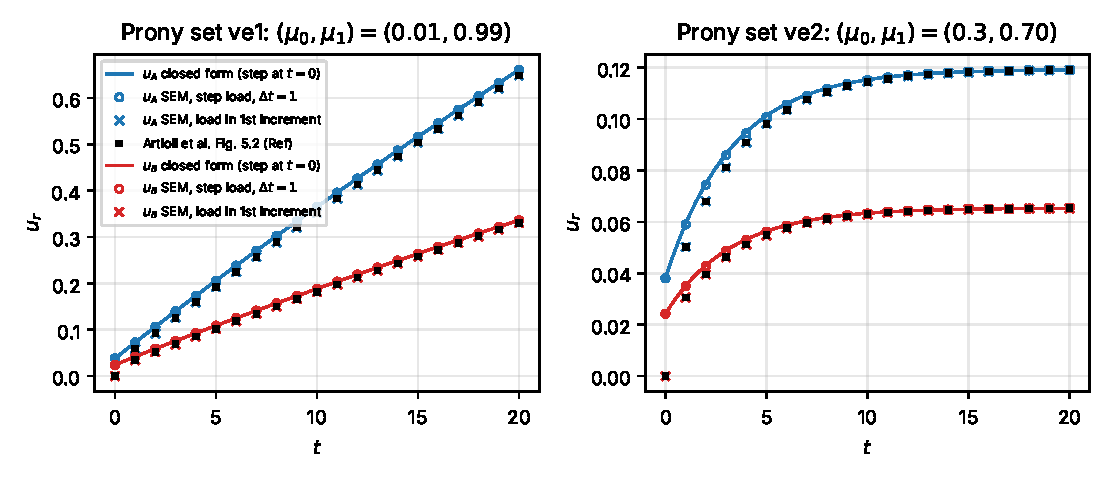
\includegraphics[width=\textwidth]{figures_quasistatic_solid/creep_curves.pdf}
\caption{Radial displacement at $A$ and $B$. Lines: closed form (Heaviside load).
Circles: SEM with the load on at $t=0^+$ and $\Delta t=1$ --- on the closed form
within the second-order time error. Crosses: SEM with the load applied in the first
increment (FEAP's convention) --- on the paper's Fig.~5.2 points (squares, read from
the vector graphics of the arXiv PDF).}
\label{fig:creep}
\end{figure}

\begin{table}[ht]
\centering
\small
\begin{tabularx}{\textwidth}{@{}Xll@{}}
\toprule
check & result & reference\\
\midrule
$t=0^+$, $u_A$ & $0.0381333412$ & Lam\'e $0.0381333333$\\
spatial error alone, $N=2,3,4,5,6$ & $2.3\!\times\!10^{-3}$, $2.5\!\times\!10^{-6}$, $6.0\!\times\!10^{-7}$, & time-discrete\\
 & $4.1\!\times\!10^{-9}$, $1.0\!\times\!10^{-9}$ & reference\\
time error, $\Delta t=1\to\tfrac18$, exponential (ve1/ve2) & rates $1.98$--$2.04$ / $1.97$--$2.00$ & closed form\\
time error, midpoint (ve1) / backward Euler (ve2) & rates $2.00$--$2.01$ / $0.91$--$0.98$ & closed form\\
quadrature-point path vs nodal path & $7\!\times\!10^{-13}$ (relative) & round-off\\
paper Fig.~5.2, $\max|u-u_{\mathrm{paper}}|$ (ve1 / ve2) & $1.1\!\times\!10^{-4}$ / $2.4\!\times\!10^{-5}$ & figure resolution\\
\bottomrule
\end{tabularx}
\caption{Verification of the viscoelastic case (\code{test/test\_viscoelastic\_cylinder.jl}, 23/23).
Errors are relative to $\max u_A$ unless stated.}
\label{tab:ve}
\end{table}

\begin{figure}[ht]
\centering
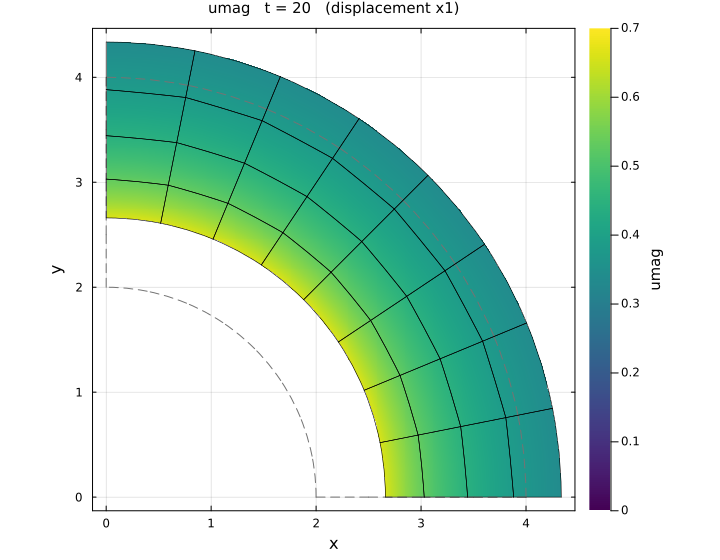
\includegraphics[width=0.55\textwidth]{figures_quasistatic_solid/ve_deformed_t20.png}
\caption{The deformed grid at $t=20$ (ve1), true scale, coloured by $|\bu|$, over the
undeformed outline (dashed): the bore has crept from $r=2$ to $2.66$. Drawn by
\code{plot\_deformed\_mesh} (\code{:lplot\_deformed}).}
\label{fig:vedef}
\end{figure}

\subsection{Elastic--perfectly plastic cylinder (the history at the quadrature points)}

The same quarter cylinder, $J_2$ with the material of Artioli et al.\ \S4.3
($E=7000$, $\nu=0.3$, $\sigma_{y0}=24.3$, no hardening), $N=4$, $8\times8$
elements, its bore displaced radially to $\delta=0.05$ in 50 increments. Up to
first yield the solution is Lam\'e's ($p_e=10.5047$); with the whole wall
flowing, the pressure levels off at the exact limit
$p_L=\frac{2}{\sqrt3}\sigma_{y0}\ln\frac ba=19.4492$ (Hill 1950).

\begin{figure}[!ht]
\centering
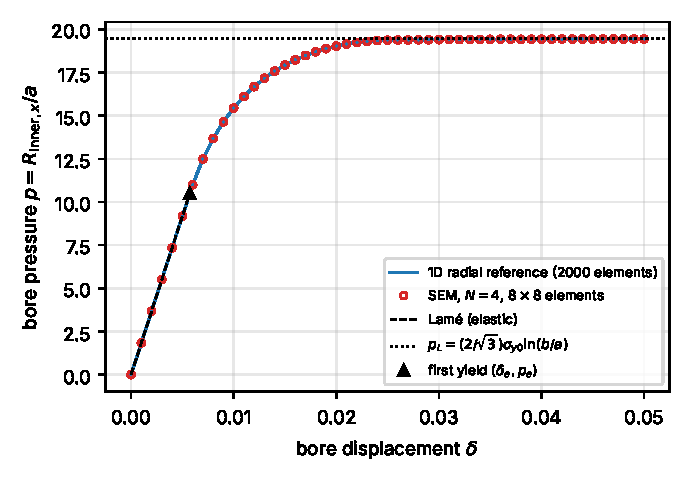
\includegraphics[width=0.6\textwidth]{figures_quasistatic_solid/plastic_pressure.pdf}\\[6pt]
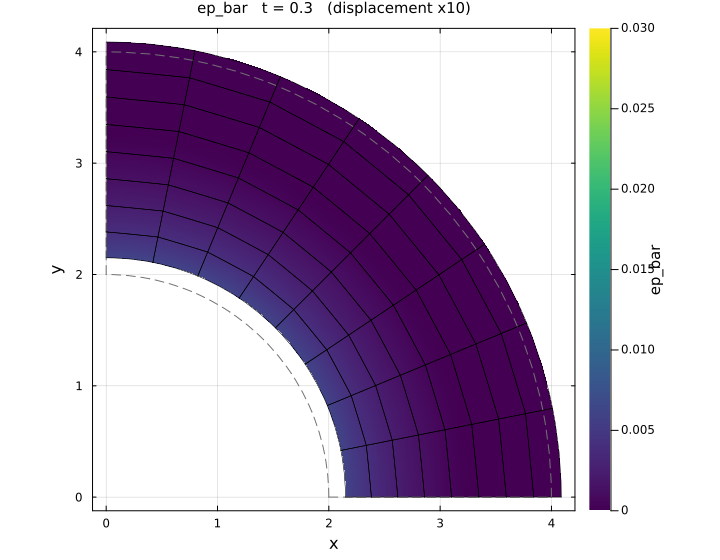
\includegraphics[width=0.325\textwidth]{figures_quasistatic_solid/pc_deformed_it4.png}\hfill
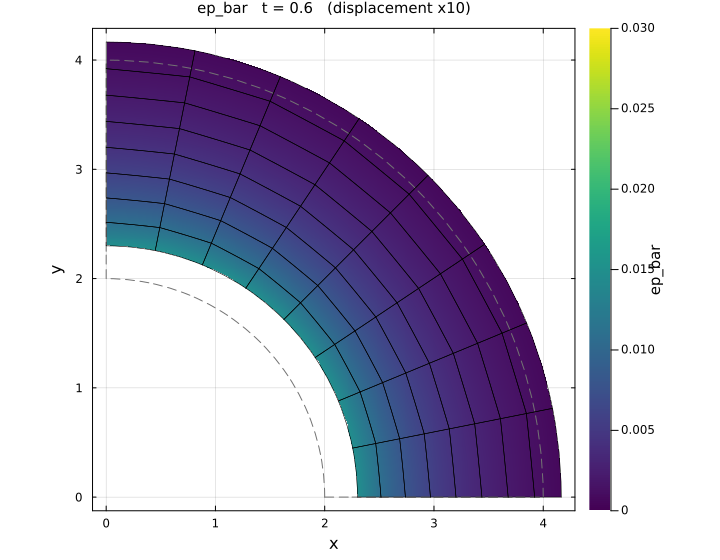
\includegraphics[width=0.325\textwidth]{figures_quasistatic_solid/pc_deformed_it7.png}\hfill
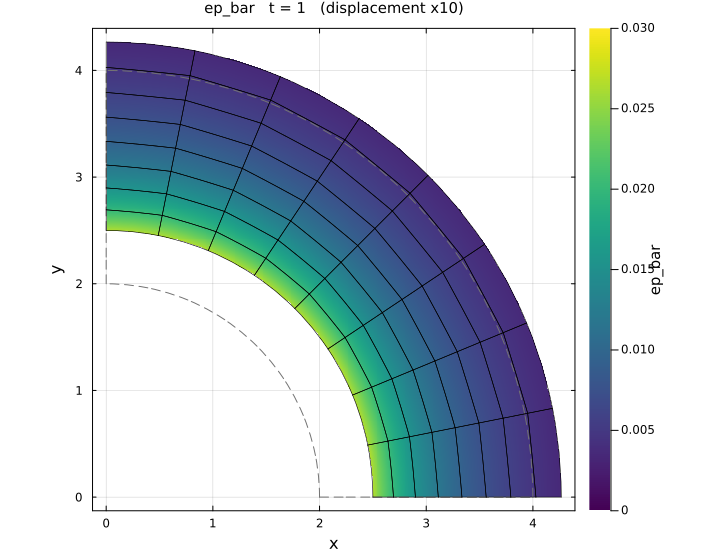
\includegraphics[width=0.325\textwidth]{figures_quasistatic_solid/pc_deformed_it11.png}
\caption{Top: bore pressure against bore displacement --- SEM, the 1D radial reference
(same constitutive routine and increments), Lam\'e and the exact limit. Bottom: the
deformed grid ($\times10$) coloured by the accumulated plastic strain $\bar e^p$, a
quadrature-point history value projected onto the nodes, at $t=0.3$, $0.6$ and $1$:
the plastic zone spreads from the bore until the whole wall has yielded.}
\label{fig:plastic}
\end{figure}

\begin{table}[ht]
\centering
\small
\begin{tabularx}{\textwidth}{@{}Xl@{}}
\toprule
check & result\\
\midrule
$J_2$ point, cyclic uniaxial strain, isotropic + kinematic hardening, vs exact & $1.3\!\times\!10^{-16}$\\
consistent tangent vs finite differences & $\le1.7\!\times\!10^{-11}$\\
bore pressure before first yield vs Lam\'e & $1.9\!\times\!10^{-7}$, $\bar e^p=0$\\
bore pressure vs 1D radial reference, all increments & $1.3\!\times\!10^{-4}\,p_L$\\
$p(\delta=0.05)$ & $19.44145$ (reference $19.44143$, $p_L=19.44917$)\\
Newton iterations per increment & $3.8$ on average, at most 5\\
\bottomrule
\end{tabularx}
\caption{Verification of the plasticity case (\code{test/test\_plastic\_cylinder.jl}, 16/16).}
\label{tab:pc}
\end{table}

\subsection{Seeing the solid deform}
Both cases write the displacement also as a vector \code{u}
(\code{:vtk\_vectors}). In ParaView: open \code{simulation.pvd}, apply
\emph{Warp By Vector} with vector \code{u} (scale 1 for the viscoelastic
cylinder, $\sim$10 for the plastic one), colour by any field (\code{szz},
\code{svm}, \code{ep\_bar}, \dots) and press \emph{Play}. Without ParaView,
\code{:lplot\_deformed => true} writes \code{deformed-<field>-it<k>.png} and
\code{deformed.gif} (Figs.~\ref{fig:vedef},~\ref{fig:plastic}).


\coderef{\jxfile{test/test_viscoelastic_cylinder.jl}{test/test\_viscoelastic\_cylinder.jl},
\jxfile{test/test_plastic_cylinder.jl}{test/test\_plastic\_cylinder.jl}.}


%==============================================================================
\section{The perforated plastic plate (\S4.3 of the paper)}\label{sec:plate}
%==============================================================================

The paper's second inelastic benchmark puts the quadrature-point path of
Step~7 through a genuinely two-dimensional plastic flow. A strip
$2L\times2H=200\times360$~mm with a central hole of diameter $2R=100$~mm, in
plane strain, made of the elastic--perfectly plastic $J_2$ material of
\S\ref{sec:constitutive} with $E=7000$~kg/mm$^2$, $\nu=0.3$,
$\sigma_{y0}=24.3$~kg/mm$^2$ and no hardening, is stretched along its length:
the normal displacement is prescribed on the symmetry lines, on the lateral
edges and on the ends, which are pulled apart by $\delta=2$~mm in 400 equal
increments. A quarter is modelled (Fig.~\ref{fig:platesetup}).
\begin{figure}[ht]
\centering
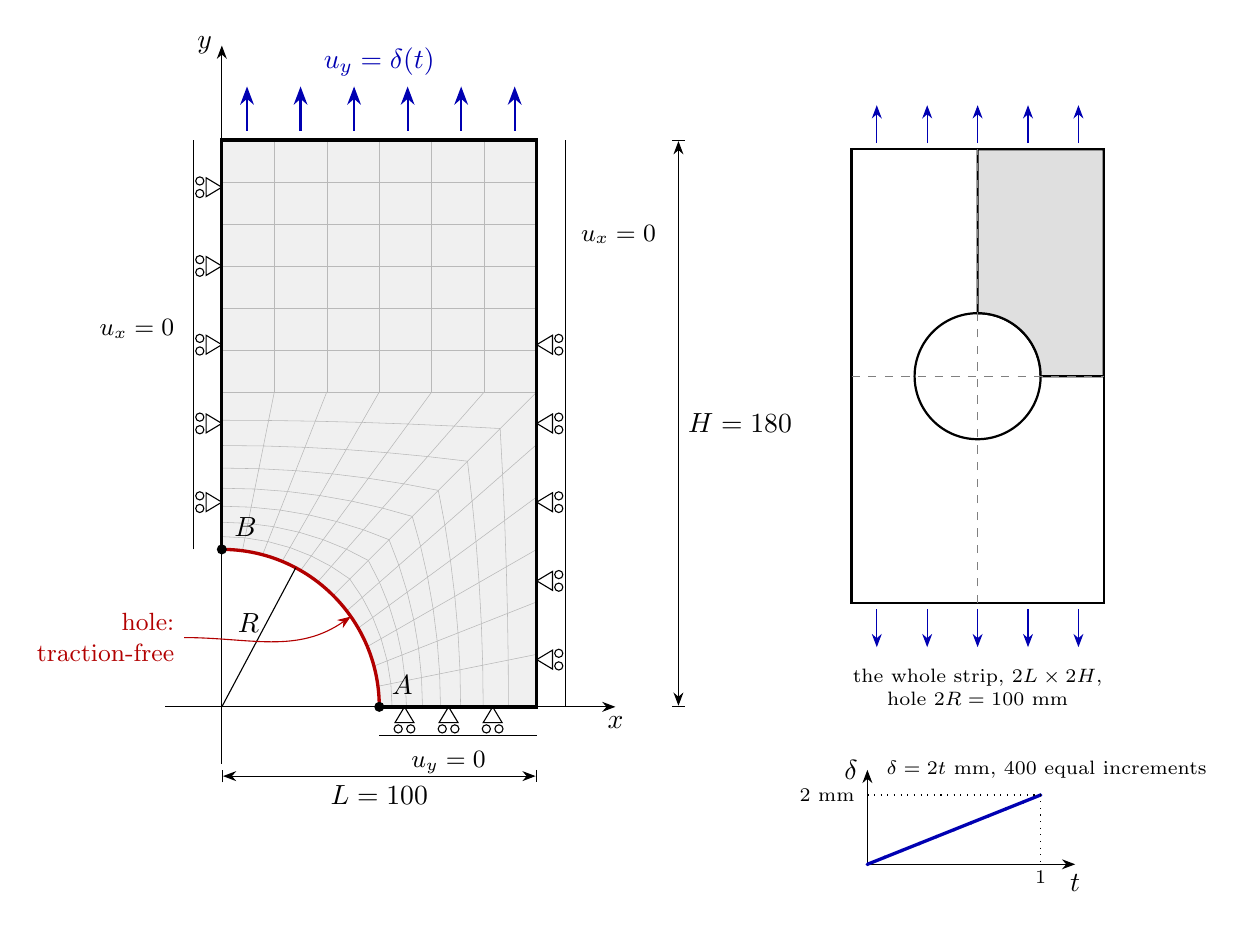
\begin{tikzpicture}[x=0.04cm,y=0.04cm,>=Stealth,
                    meshline/.style={gray!55,very thin}]
  \def\L{100}\def\H{180}\def\R{50}
  % body and its grid
  \fill[gray!12] (\R,0) -- (\L,0) -- (\L,\H) -- (0,\H) -- (0,\R) arc[start angle=90,end angle=0,radius=\R] -- cycle;
  % 132 quadrilaterals, 290 edges, from quarter_plate_hole_132.msh
\draw[meshline] (50.0000,0.0000) -- (54.0651,0.0000);
\draw[meshline] (50.0000,0.0000) arc[start angle=0.0000,end angle=7.5000,radius=50.0000];
\draw[meshline] (100.0000,0.0000) -- (91.0133,0.0000);
\draw[meshline] (100.0000,0.0000) -- (100.0000,16.6667);
\draw[meshline] (100.0000,100.0000) -- (88.3811,88.3811);
\draw[meshline] (100.0000,100.0000) -- (100.0000,83.3333);
\draw[meshline] (100.0000,100.0000) -- (83.3333,100.0000);
\draw[meshline] (100.0000,100.0000) -- (100.0000,113.3333);
\draw[meshline] (35.3553,35.3553) -- (40.6111,40.6111);
\draw[meshline] (35.3553,35.3553) arc[start angle=45.0000,end angle=37.5000,radius=50.0000];
\draw[meshline] (35.3553,35.3553) arc[start angle=45.0000,end angle=52.5000,radius=50.0000];
\draw[meshline] (0.0000,100.0000) -- (0.0000,91.0133);
\draw[meshline] (0.0000,100.0000) -- (16.6667,100.0000);
\draw[meshline] (0.0000,100.0000) -- (0.0000,113.3333);
\draw[meshline] (0.0000,50.0000) -- (0.0000,54.0651);
\draw[meshline] (0.0000,50.0000) arc[start angle=90.0000,end angle=82.5000,radius=50.0000];
\draw[meshline] (100.0000,180.0000) -- (100.0000,166.6667);
\draw[meshline] (100.0000,180.0000) -- (83.3333,180.0000);
\draw[meshline] (0.0000,180.0000) -- (16.6667,180.0000);
\draw[meshline] (0.0000,180.0000) -- (0.0000,166.6667);
\draw[meshline] (54.0651,0.0000) -- (58.6181,0.0000);
\draw[meshline] (54.0651,0.0000) -- (53.6722,7.3507);
\draw[meshline] (58.6181,0.0000) -- (63.7174,0.0000);
\draw[meshline] (58.6181,0.0000) -- (58.2641,8.2741);
\draw[meshline] (63.7174,0.0000) -- (69.4286,0.0000);
\draw[meshline] (63.7174,0.0000) -- (63.4070,9.3083);
\draw[meshline] (69.4286,0.0000) -- (75.8252,0.0000);
\draw[meshline] (69.4286,0.0000) -- (69.1671,10.4666);
\draw[meshline] (75.8252,0.0000) -- (82.9894,0.0000);
\draw[meshline] (75.8252,0.0000) -- (75.6184,11.7639);
\draw[meshline] (82.9894,0.0000) -- (91.0133,0.0000);
\draw[meshline] (82.9894,0.0000) -- (82.8439,13.2168);
\draw[meshline] (91.0133,0.0000) -- (90.9364,14.8441);
\draw[meshline] (40.6111,40.6111) -- (46.4976,46.4976);
\draw[meshline] (40.6111,40.6111) -- (44.5729,34.7386);
\draw[meshline] (40.6111,40.6111) -- (34.7386,44.5729);
\draw[meshline] (46.4976,46.4976) -- (53.0905,53.0905);
\draw[meshline] (46.4976,46.4976) -- (50.0667,39.5552);
\draw[meshline] (46.4976,46.4976) -- (39.5552,50.0667);
\draw[meshline] (53.0905,53.0905) -- (60.4745,60.4745);
\draw[meshline] (53.0905,53.0905) -- (56.2197,44.9498);
\draw[meshline] (53.0905,53.0905) -- (44.9498,56.2197);
\draw[meshline] (60.4745,60.4745) -- (68.7446,68.7446);
\draw[meshline] (60.4745,60.4745) -- (63.1112,50.9917);
\draw[meshline] (60.4745,60.4745) -- (50.9917,63.1112);
\draw[meshline] (68.7446,68.7446) -- (78.0071,78.0071);
\draw[meshline] (68.7446,68.7446) -- (70.8296,57.7587);
\draw[meshline] (68.7446,68.7446) -- (57.7587,70.8296);
\draw[meshline] (78.0071,78.0071) -- (88.3811,88.3811);
\draw[meshline] (78.0071,78.0071) -- (79.4742,65.3377);
\draw[meshline] (78.0071,78.0071) -- (65.3377,79.4742);
\draw[meshline] (88.3811,88.3811) -- (89.1562,73.8262);
\draw[meshline] (88.3811,88.3811) -- (73.8262,89.1562);
\draw[meshline] (0.0000,54.0651) -- (0.0000,58.6181);
\draw[meshline] (0.0000,54.0651) -- (7.3507,53.6722);
\draw[meshline] (0.0000,58.6181) -- (0.0000,63.7174);
\draw[meshline] (0.0000,58.6181) -- (8.2741,58.2641);
\draw[meshline] (0.0000,63.7174) -- (0.0000,69.4286);
\draw[meshline] (0.0000,63.7174) -- (9.3083,63.4070);
\draw[meshline] (0.0000,69.4286) -- (0.0000,75.8252);
\draw[meshline] (0.0000,69.4286) -- (10.4666,69.1671);
\draw[meshline] (0.0000,75.8252) -- (0.0000,82.9894);
\draw[meshline] (0.0000,75.8252) -- (11.7639,75.6184);
\draw[meshline] (0.0000,82.9894) -- (0.0000,91.0133);
\draw[meshline] (0.0000,82.9894) -- (13.2168,82.8439);
\draw[meshline] (0.0000,91.0133) -- (14.8441,90.9364);
\draw[meshline] (49.5722,6.5263) arc[start angle=7.5000,end angle=15.0000,radius=50.0000];
\draw[meshline] (49.5722,6.5263) -- (53.6722,7.3507);
\draw[meshline] (48.2963,12.9410) arc[start angle=15.0000,end angle=22.5000,radius=50.0000];
\draw[meshline] (48.2963,12.9410) -- (52.4999,14.5989);
\draw[meshline] (46.1940,19.1342) arc[start angle=22.5000,end angle=30.0000,radius=50.0000];
\draw[meshline] (46.1940,19.1342) -- (50.5686,21.6437);
\draw[meshline] (43.3013,25.0000) arc[start angle=30.0000,end angle=37.5000,radius=50.0000];
\draw[meshline] (43.3013,25.0000) -- (47.9110,28.3876);
\draw[meshline] (39.6677,30.4381) -- (44.5729,34.7386);
\draw[meshline] (30.4381,39.6677) arc[start angle=52.5000,end angle=60.0000,radius=50.0000];
\draw[meshline] (30.4381,39.6677) -- (34.7386,44.5729);
\draw[meshline] (25.0000,43.3013) arc[start angle=60.0000,end angle=67.5000,radius=50.0000];
\draw[meshline] (25.0000,43.3013) -- (28.3876,47.9110);
\draw[meshline] (19.1342,46.1940) arc[start angle=67.5000,end angle=75.0000,radius=50.0000];
\draw[meshline] (19.1342,46.1940) -- (21.6437,50.5686);
\draw[meshline] (12.9410,48.2963) arc[start angle=75.0000,end angle=82.5000,radius=50.0000];
\draw[meshline] (12.9410,48.2963) -- (14.5989,52.4999);
\draw[meshline] (6.5263,49.5722) -- (7.3507,53.6722);
\draw[meshline] (100.0000,16.6667) -- (100.0000,33.3333);
\draw[meshline] (100.0000,16.6667) -- (90.9364,14.8441);
\draw[meshline] (100.0000,33.3333) -- (100.0000,50.0000);
\draw[meshline] (100.0000,33.3333) -- (90.7071,29.6681);
\draw[meshline] (100.0000,50.0000) -- (100.0000,66.6667);
\draw[meshline] (100.0000,50.0000) -- (90.3292,44.4523);
\draw[meshline] (100.0000,66.6667) -- (100.0000,83.3333);
\draw[meshline] (100.0000,66.6667) -- (89.8093,59.1777);
\draw[meshline] (100.0000,83.3333) -- (89.1562,73.8262);
\draw[meshline] (83.3333,100.0000) -- (66.6667,100.0000);
\draw[meshline] (83.3333,100.0000) -- (73.8262,89.1562);
\draw[meshline] (83.3333,100.0000) -- (83.3333,113.3333);
\draw[meshline] (66.6667,100.0000) -- (50.0000,100.0000);
\draw[meshline] (66.6667,100.0000) -- (59.1777,89.8093);
\draw[meshline] (66.6667,100.0000) -- (66.6667,113.3333);
\draw[meshline] (50.0000,100.0000) -- (33.3333,100.0000);
\draw[meshline] (50.0000,100.0000) -- (44.4523,90.3292);
\draw[meshline] (50.0000,100.0000) -- (50.0000,113.3333);
\draw[meshline] (33.3333,100.0000) -- (16.6667,100.0000);
\draw[meshline] (33.3333,100.0000) -- (29.6681,90.7071);
\draw[meshline] (33.3333,100.0000) -- (33.3333,113.3333);
\draw[meshline] (16.6667,100.0000) -- (14.8441,90.9364);
\draw[meshline] (16.6667,100.0000) -- (16.6667,113.3333);
\draw[meshline] (100.0000,113.3333) -- (100.0000,126.6667);
\draw[meshline] (100.0000,113.3333) -- (83.3333,113.3333);
\draw[meshline] (100.0000,126.6667) -- (100.0000,140.0000);
\draw[meshline] (100.0000,126.6667) -- (83.3333,126.6667);
\draw[meshline] (100.0000,140.0000) -- (100.0000,153.3333);
\draw[meshline] (100.0000,140.0000) -- (83.3333,140.0000);
\draw[meshline] (100.0000,153.3333) -- (100.0000,166.6667);
\draw[meshline] (100.0000,153.3333) -- (83.3333,153.3333);
\draw[meshline] (100.0000,166.6667) -- (83.3333,166.6667);
\draw[meshline] (83.3333,180.0000) -- (66.6667,180.0000);
\draw[meshline] (83.3333,180.0000) -- (83.3333,166.6667);
\draw[meshline] (66.6667,180.0000) -- (50.0000,180.0000);
\draw[meshline] (66.6667,180.0000) -- (66.6667,166.6667);
\draw[meshline] (50.0000,180.0000) -- (33.3333,180.0000);
\draw[meshline] (50.0000,180.0000) -- (50.0000,166.6667);
\draw[meshline] (33.3333,180.0000) -- (16.6667,180.0000);
\draw[meshline] (33.3333,180.0000) -- (33.3333,166.6667);
\draw[meshline] (16.6667,180.0000) -- (16.6667,166.6667);
\draw[meshline] (0.0000,113.3333) -- (0.0000,126.6667);
\draw[meshline] (0.0000,113.3333) -- (16.6667,113.3333);
\draw[meshline] (0.0000,126.6667) -- (0.0000,140.0000);
\draw[meshline] (0.0000,126.6667) -- (16.6667,126.6667);
\draw[meshline] (0.0000,140.0000) -- (0.0000,153.3333);
\draw[meshline] (0.0000,140.0000) -- (16.6667,140.0000);
\draw[meshline] (0.0000,153.3333) -- (0.0000,166.6667);
\draw[meshline] (0.0000,153.3333) -- (16.6667,153.3333);
\draw[meshline] (0.0000,166.6667) -- (16.6667,166.6667);
\draw[meshline] (53.6722,7.3507) -- (52.4999,14.5989);
\draw[meshline] (53.6722,7.3507) -- (58.2641,8.2741);
\draw[meshline] (52.4999,14.5989) -- (50.5686,21.6437);
\draw[meshline] (52.4999,14.5989) -- (57.2080,16.4558);
\draw[meshline] (50.5686,21.6437) -- (47.9110,28.3876);
\draw[meshline] (50.5686,21.6437) -- (55.4681,24.4543);
\draw[meshline] (47.9110,28.3876) -- (44.5729,34.7386);
\draw[meshline] (47.9110,28.3876) -- (53.0740,32.1818);
\draw[meshline] (44.5729,34.7386) -- (50.0667,39.5552);
\draw[meshline] (58.2641,8.2741) -- (57.2080,16.4558);
\draw[meshline] (58.2641,8.2741) -- (63.4070,9.3083);
\draw[meshline] (57.2080,16.4558) -- (55.4681,24.4543);
\draw[meshline] (57.2080,16.4558) -- (62.4811,18.5356);
\draw[meshline] (55.4681,24.4543) -- (53.0740,32.1818);
\draw[meshline] (55.4681,24.4543) -- (60.9556,27.6022);
\draw[meshline] (53.0740,32.1818) -- (50.0667,39.5552);
\draw[meshline] (53.0740,32.1818) -- (58.8565,36.4312);
\draw[meshline] (50.0667,39.5552) -- (56.2197,44.9498);
\draw[meshline] (63.4070,9.3083) -- (62.4811,18.5356);
\draw[meshline] (63.4070,9.3083) -- (69.1671,10.4666);
\draw[meshline] (62.4811,18.5356) -- (60.9556,27.6022);
\draw[meshline] (62.4811,18.5356) -- (68.3870,20.8649);
\draw[meshline] (60.9556,27.6022) -- (58.8565,36.4312);
\draw[meshline] (60.9556,27.6022) -- (67.1015,31.1278);
\draw[meshline] (58.8565,36.4312) -- (56.2197,44.9498);
\draw[meshline] (58.8565,36.4312) -- (65.3329,41.1905);
\draw[meshline] (56.2197,44.9498) -- (63.1112,50.9917);
\draw[meshline] (69.1671,10.4666) -- (68.3870,20.8649);
\draw[meshline] (69.1671,10.4666) -- (75.6184,11.7639);
\draw[meshline] (68.3870,20.8649) -- (67.1015,31.1278);
\draw[meshline] (68.3870,20.8649) -- (75.0015,23.4737);
\draw[meshline] (67.1015,31.1278) -- (65.3329,41.1905);
\draw[meshline] (67.1015,31.1278) -- (73.9850,35.0765);
\draw[meshline] (65.3329,41.1905) -- (63.1112,50.9917);
\draw[meshline] (65.3329,41.1905) -- (72.5864,46.5210);
\draw[meshline] (63.1112,50.9917) -- (70.8296,57.7587);
\draw[meshline] (75.6184,11.7639) -- (75.0015,23.4737);
\draw[meshline] (75.6184,11.7639) -- (82.8439,13.2168);
\draw[meshline] (75.0015,23.4737) -- (73.9850,35.0765);
\draw[meshline] (75.0015,23.4737) -- (82.4098,26.3956);
\draw[meshline] (73.9850,35.0765) -- (72.5864,46.5210);
\draw[meshline] (73.9850,35.0765) -- (81.6945,39.4991);
\draw[meshline] (72.5864,46.5210) -- (70.8296,57.7587);
\draw[meshline] (72.5864,46.5210) -- (80.7104,52.4912);
\draw[meshline] (70.8296,57.7587) -- (79.4742,65.3377);
\draw[meshline] (82.8439,13.2168) -- (82.4098,26.3956);
\draw[meshline] (82.8439,13.2168) -- (90.9364,14.8441);
\draw[meshline] (82.4098,26.3956) -- (81.6945,39.4991);
\draw[meshline] (82.4098,26.3956) -- (90.7071,29.6681);
\draw[meshline] (81.6945,39.4991) -- (80.7104,52.4912);
\draw[meshline] (81.6945,39.4991) -- (90.3292,44.4523);
\draw[meshline] (80.7104,52.4912) -- (79.4742,65.3377);
\draw[meshline] (80.7104,52.4912) -- (89.8093,59.1777);
\draw[meshline] (79.4742,65.3377) -- (89.1562,73.8262);
\draw[meshline] (90.9364,14.8441) -- (90.7071,29.6681);
\draw[meshline] (90.7071,29.6681) -- (90.3292,44.4523);
\draw[meshline] (90.3292,44.4523) -- (89.8093,59.1777);
\draw[meshline] (89.8093,59.1777) -- (89.1562,73.8262);
\draw[meshline] (34.7386,44.5729) -- (28.3876,47.9110);
\draw[meshline] (34.7386,44.5729) -- (39.5552,50.0667);
\draw[meshline] (28.3876,47.9110) -- (21.6437,50.5686);
\draw[meshline] (28.3876,47.9110) -- (32.1818,53.0740);
\draw[meshline] (21.6437,50.5686) -- (14.5989,52.4999);
\draw[meshline] (21.6437,50.5686) -- (24.4543,55.4681);
\draw[meshline] (14.5989,52.4999) -- (7.3507,53.6722);
\draw[meshline] (14.5989,52.4999) -- (16.4558,57.2080);
\draw[meshline] (7.3507,53.6722) -- (8.2741,58.2641);
\draw[meshline] (39.5552,50.0667) -- (32.1818,53.0740);
\draw[meshline] (39.5552,50.0667) -- (44.9498,56.2197);
\draw[meshline] (32.1818,53.0740) -- (24.4543,55.4681);
\draw[meshline] (32.1818,53.0740) -- (36.4312,58.8565);
\draw[meshline] (24.4543,55.4681) -- (16.4558,57.2080);
\draw[meshline] (24.4543,55.4681) -- (27.6022,60.9556);
\draw[meshline] (16.4558,57.2080) -- (8.2741,58.2641);
\draw[meshline] (16.4558,57.2080) -- (18.5356,62.4811);
\draw[meshline] (8.2741,58.2641) -- (9.3083,63.4070);
\draw[meshline] (44.9498,56.2197) -- (36.4312,58.8565);
\draw[meshline] (44.9498,56.2197) -- (50.9917,63.1112);
\draw[meshline] (36.4312,58.8565) -- (27.6022,60.9556);
\draw[meshline] (36.4312,58.8565) -- (41.1905,65.3329);
\draw[meshline] (27.6022,60.9556) -- (18.5356,62.4811);
\draw[meshline] (27.6022,60.9556) -- (31.1278,67.1015);
\draw[meshline] (18.5356,62.4811) -- (9.3083,63.4070);
\draw[meshline] (18.5356,62.4811) -- (20.8649,68.3870);
\draw[meshline] (9.3083,63.4070) -- (10.4666,69.1671);
\draw[meshline] (50.9917,63.1112) -- (41.1905,65.3329);
\draw[meshline] (50.9917,63.1112) -- (57.7587,70.8296);
\draw[meshline] (41.1905,65.3329) -- (31.1278,67.1015);
\draw[meshline] (41.1905,65.3329) -- (46.5210,72.5864);
\draw[meshline] (31.1278,67.1015) -- (20.8649,68.3870);
\draw[meshline] (31.1278,67.1015) -- (35.0765,73.9850);
\draw[meshline] (20.8649,68.3870) -- (10.4666,69.1671);
\draw[meshline] (20.8649,68.3870) -- (23.4737,75.0015);
\draw[meshline] (10.4666,69.1671) -- (11.7639,75.6184);
\draw[meshline] (57.7587,70.8296) -- (46.5210,72.5864);
\draw[meshline] (57.7587,70.8296) -- (65.3377,79.4742);
\draw[meshline] (46.5210,72.5864) -- (35.0765,73.9850);
\draw[meshline] (46.5210,72.5864) -- (52.4912,80.7104);
\draw[meshline] (35.0765,73.9850) -- (23.4737,75.0015);
\draw[meshline] (35.0765,73.9850) -- (39.4991,81.6945);
\draw[meshline] (23.4737,75.0015) -- (11.7639,75.6184);
\draw[meshline] (23.4737,75.0015) -- (26.3956,82.4098);
\draw[meshline] (11.7639,75.6184) -- (13.2168,82.8439);
\draw[meshline] (65.3377,79.4742) -- (52.4912,80.7104);
\draw[meshline] (65.3377,79.4742) -- (73.8262,89.1562);
\draw[meshline] (52.4912,80.7104) -- (39.4991,81.6945);
\draw[meshline] (52.4912,80.7104) -- (59.1777,89.8093);
\draw[meshline] (39.4991,81.6945) -- (26.3956,82.4098);
\draw[meshline] (39.4991,81.6945) -- (44.4523,90.3292);
\draw[meshline] (26.3956,82.4098) -- (13.2168,82.8439);
\draw[meshline] (26.3956,82.4098) -- (29.6681,90.7071);
\draw[meshline] (13.2168,82.8439) -- (14.8441,90.9364);
\draw[meshline] (73.8262,89.1562) -- (59.1777,89.8093);
\draw[meshline] (59.1777,89.8093) -- (44.4523,90.3292);
\draw[meshline] (44.4523,90.3292) -- (29.6681,90.7071);
\draw[meshline] (29.6681,90.7071) -- (14.8441,90.9364);
\draw[meshline] (83.3333,113.3333) -- (83.3333,126.6667);
\draw[meshline] (83.3333,113.3333) -- (66.6667,113.3333);
\draw[meshline] (83.3333,126.6667) -- (83.3333,140.0000);
\draw[meshline] (83.3333,126.6667) -- (66.6667,126.6667);
\draw[meshline] (83.3333,140.0000) -- (83.3333,153.3333);
\draw[meshline] (83.3333,140.0000) -- (66.6667,140.0000);
\draw[meshline] (83.3333,153.3333) -- (83.3333,166.6667);
\draw[meshline] (83.3333,153.3333) -- (66.6667,153.3333);
\draw[meshline] (83.3333,166.6667) -- (66.6667,166.6667);
\draw[meshline] (66.6667,113.3333) -- (66.6667,126.6667);
\draw[meshline] (66.6667,113.3333) -- (50.0000,113.3333);
\draw[meshline] (66.6667,126.6667) -- (66.6667,140.0000);
\draw[meshline] (66.6667,126.6667) -- (50.0000,126.6667);
\draw[meshline] (66.6667,140.0000) -- (66.6667,153.3333);
\draw[meshline] (66.6667,140.0000) -- (50.0000,140.0000);
\draw[meshline] (66.6667,153.3333) -- (66.6667,166.6667);
\draw[meshline] (66.6667,153.3333) -- (50.0000,153.3333);
\draw[meshline] (66.6667,166.6667) -- (50.0000,166.6667);
\draw[meshline] (50.0000,113.3333) -- (50.0000,126.6667);
\draw[meshline] (50.0000,113.3333) -- (33.3333,113.3333);
\draw[meshline] (50.0000,126.6667) -- (50.0000,140.0000);
\draw[meshline] (50.0000,126.6667) -- (33.3333,126.6667);
\draw[meshline] (50.0000,140.0000) -- (50.0000,153.3333);
\draw[meshline] (50.0000,140.0000) -- (33.3333,140.0000);
\draw[meshline] (50.0000,153.3333) -- (50.0000,166.6667);
\draw[meshline] (50.0000,153.3333) -- (33.3333,153.3333);
\draw[meshline] (50.0000,166.6667) -- (33.3333,166.6667);
\draw[meshline] (33.3333,113.3333) -- (33.3333,126.6667);
\draw[meshline] (33.3333,113.3333) -- (16.6667,113.3333);
\draw[meshline] (33.3333,126.6667) -- (33.3333,140.0000);
\draw[meshline] (33.3333,126.6667) -- (16.6667,126.6667);
\draw[meshline] (33.3333,140.0000) -- (33.3333,153.3333);
\draw[meshline] (33.3333,140.0000) -- (16.6667,140.0000);
\draw[meshline] (33.3333,153.3333) -- (33.3333,166.6667);
\draw[meshline] (33.3333,153.3333) -- (16.6667,153.3333);
\draw[meshline] (33.3333,166.6667) -- (16.6667,166.6667);
\draw[meshline] (16.6667,113.3333) -- (16.6667,126.6667);
\draw[meshline] (16.6667,126.6667) -- (16.6667,140.0000);
\draw[meshline] (16.6667,140.0000) -- (16.6667,153.3333);
\draw[meshline] (16.6667,153.3333) -- (16.6667,166.6667);

  % boundaries
  \draw[very thick] (\R,0) -- (\L,0) -- (\L,\H) -- (0,\H) -- (0,\R);
  \draw[very thick,red!70!black] (0,\R) arc[start angle=90,end angle=0,radius=\R];
  % imposed displacement on the top edge
  \foreach \x in {8,25,...,93}{ \draw[->,blue!70!black,thick] (\x,\H+3) -- (\x,\H+17); }
  \node[blue!70!black,anchor=south] at (50,\H+17) {$u_y=\delta(t)$};
  % rollers: x = 0 above the hole and x = L (u_x = 0)
  \foreach \y in {65,90,...,165}{
     \draw (0,\y) -- (-5,\y-3) -- (-5,\y+3) -- cycle; \draw (-7,\y-2) circle (1.3); \draw (-7,\y+2) circle (1.3);
     \draw (\L,\y-50) -- (\L+5,\y-53) -- (\L+5,\y-47) -- cycle; \draw (\L+7,\y-52) circle (1.3); \draw (\L+7,\y-48) circle (1.3);}
  \draw (-9,\R) -- (-9,\H);
  \draw (\L+9,0) -- (\L+9,\H);
  % rollers: y = 0 right of the hole (u_y = 0)
  \foreach \x in {58,72,86}{ \draw (\x,0) -- (\x-3,-5) -- (\x+3,-5) -- cycle; \draw (\x-2,-7) circle (1.3); \draw (\x+2,-7) circle (1.3);}
  \draw (\R,-9) -- (\L,-9);
  % axes and points
  \draw[->] (-18,0) -- (\L+25,0) node[below] {$x$};
  \draw[->] (0,-18) -- (0,\H+30) node[left] {$y$};
  \fill (\R,0) circle (1.6) node[above right=1pt] {$A$};
  \fill (0,\R) circle (1.6) node[above right=1pt] {$B$};
  % dimensions
  \draw[|<->|,thin] (0,-22) -- node[below] {$L=100$} (\L,-22);
  \draw[|<->|,thin] (\L+45,0) -- node[right] {$H=180$} (\L+45,\H);
  \draw[thin] (0,0) -- node[pos=0.6,left=-1pt] {$R$} ({\R*cos(62)},{\R*sin(62)});
  % labels
  \node[font=\small,red!70!black,align=right,anchor=east] (hole) at (-12,22) {hole:\\ traction-free};
  \draw[->,thin,red!70!black] (hole.east) to[out=0,in=215] (35:\R);
  \node[font=\small,anchor=east,align=right] at (-12,120) {$u_x=0$};
  \node[font=\small,anchor=west,align=left] at (\L+11,150) {$u_x=0$};
  \node[font=\small,anchor=north] at (72,-11) {$u_y=0$};
  % the whole strip, the modelled quarter shaded
  \begin{scope}[shift={(240,105)},x=0.016cm,y=0.016cm]
    \draw[thick] (-100,-180) rectangle (100,180);
    \draw[thick] (0,0) circle (50);
    \fill[gray!25] (50,0) -- (100,0) -- (100,180) -- (0,180) -- (0,50) arc[start angle=90,end angle=0,radius=50] -- cycle;
    \draw[thick] (50,0) -- (100,0) -- (100,180) -- (0,180) -- (0,50) arc[start angle=90,end angle=0,radius=50];
    \draw[dashed,gray] (-100,0) -- (100,0); \draw[dashed,gray] (0,-180) -- (0,180);
    \foreach \x in {-80,-40,...,80}{ \draw[->,blue!70!black] (\x,185) -- (\x,215); \draw[->,blue!70!black] (\x,-185) -- (\x,-215);}
    \node[font=\scriptsize,align=center,anchor=north] at (0,-225) {the whole strip, $2L\times2H$,\\ hole $2R=100$ mm};
  \end{scope}
  % load history
  \begin{scope}[shift={(205,-50)}]
    \draw[->] (0,0) -- (66,0) node[below] {$t$};
    \draw[->] (0,0) -- (0,30) node[left] {$\delta$};
    \draw[very thick,blue!70!black] (0,0) -- (55,22);
    \foreach \k in {0,...,10}{ \fill[blue!70!black] (5.5*\k,2.2*\k) circle (0.6); }
    \node[font=\scriptsize] at (55,-4) {$1$};
    \node[font=\scriptsize,anchor=east] at (-1,22) {2 mm};
    \draw[dotted] (0,22) -- (55,22) -- (55,0);
    \node[font=\scriptsize,anchor=west,align=left] at (3,30) {$\delta=2t$ mm, 400 equal increments};
  \end{scope}
\end{tikzpicture}
\caption{The perforated plate. Left: the modelled quarter, plane strain, with its
spectral-element grid --- 132 quadrilaterals in three structured blocks graded
towards the hole, the hole curved onto its circle --- and the boundary conditions:
the top edge pulled up by $\delta(t)$ (tangentially free), the lateral edge and
the two symmetry lines on rollers, the hole traction-free. $A=(R,0)$ and $B=(0,R)$
are the points of Table~1 of the paper. Right: the whole strip, the quarter shaded;
the imposed displacement, $\delta=2t$ mm in 400 equal increments.}
\label{fig:platesetup}
\end{figure}

\begin{table}[ht]
\centering
\small
\begin{tabularx}{\textwidth}{@{}lXl@{}}
\toprule
tag & where & condition (\code{user\_solid\_bc})\\
\midrule
\code{top} & $y=H$ & $u_y=\delta(t)=2t$~mm, $u_x$ free (the load)\\
\code{right} & $x=L$ & $u_x=0$, $u_y$ free (the lateral restraint)\\
\code{left} & $x=0$, $y\ge R$ & $u_x=0$ (symmetry)\\
\code{bottom} & $y=0$, $x\ge R$ & $u_y=0$ (symmetry)\\
\code{hole} & $r=R$ & traction-free\\
\midrule
\multicolumn{3}{@{}l}{grid: $132$ quadrilaterals, $N=4$: $2217$ nodes, $4434$ DOFs ($164$ constrained); $t\in[0,1]$, $\Delta t=1/400$}\\
\bottomrule
\end{tabularx}
\caption{Boundary conditions and discretisation of the perforated plate. The
material is rate independent, so $t$ is a load parameter. The corners join a
$u_x$ and a $u_y$ condition, so every constrained component belongs to one tag
and the reaction on \code{top} is the force the top edge carries.}
\label{tab:platebc}
\end{table}

\coderef{the case \jxfile{problems/Elasticity/perforated_plate2d}{problems/Elasticity/perforated\_plate2d}:
deck \jx{problems/Elasticity/perforated_plate2d/user_inputs.jl}{13}{user\_inputs},
material and geometry \jx{problems/Elasticity/perforated_plate2d/user_flux.jl}{27}{perforated\_plate\_properties},
boundary conditions \jx{problems/Elasticity/perforated_plate2d/user_bc.jl}{19}{user\_solid\_bc},
the paper's numbers \jx{problems/Elasticity/perforated_plate2d/user_analytic.jl}{15}{perforated\_plate\_paper\_reference};
grid \jx{problems/Elasticity/make_meshes.py}{135}{structured\_perforated\_plate}
(three transfinite blocks graded towards the hole, the hole curved back onto its
circle by \code{:exact\_geometry}).}

\paragraph{Discretisation and solution.} Nothing is specific to the plate: the
grid, basis and metric terms of Steps~1--2, the tangent of Step~3 rebuilt and
refactorised at every Newton iteration, the prescribed top displacement as a
time-dependent Dirichlet value of Step~5, the history $\{\be^p,\bar e^p\}$ at
each of the $132\times25$ quadrature points, and Algorithm~\ref{alg:newton} at
every increment. The reactions are the residual on the constrained components,
$\mathbf R_c=\mathbf f^{\mathrm{int}}_c-\mathbf f^{\mathrm{ext}}_c$, written as
the nodal fields \code{rx}, \code{ry} (zero elsewhere) and summed per tag into
\code{solid\_history.csv}. Starting from the unloaded state
(\code{:linitial\_elastic\_solve => false}) the whole run takes
about three minutes, VTK output every four increments included, on one core.
\coderef{reaction fields \jx{src/kernel/solvers/quasistatic_solid.jl}{1001}{rx, ry};
per tag \jx{src/kernel/solvers/quasistatic_solid.jl}{1049}{reactions}.}

\paragraph{Results.} Table~\ref{tab:plate} compares the displacements of $A$
and $B$ at the end of the loading with the paper's Table~1: Jexpresso's
order-4 elements land on the paper's reference solution (an overkill mixed
$u$--$p$--$\varepsilon^v$ finite-element computation) to $0.07\,\%$ and
$0.27\,\%$, closer than any of the paper's quadratic VEM or FEM. The reaction on
the top edge (Fig.~\ref{fig:platereaction}) rises elastically, bends as the
plastic zone spreads from the hole (Fig.~\ref{fig:platezone}) across the
ligament to the lateral edge, and levels off at the limit load. Over the
elastic steps the paper's reaction sums are exactly ten times Jexpresso's
($9.990\text{--}10.010$ across its five methods) while the displacements agree: the
paper's force is that of a plate 10~mm thick, a thickness it does not state,
and Jexpresso's force per unit thickness is multiplied by 10 to be drawn on the
paper's axes. At the end of the loading it is $19\,507$~kg against the paper's
$19\,557$--$19\,755$~kg, $0.25$--$1.25\,\%$ below its quadratic methods ---
displacement-based elements approach a limit load from above --- and nearly
flat: it rises by $0.05\,\%$ from step 200 to step 400, the paper's curves by
$0.16$--$0.70\,\%$.

\begin{table}[ht]
\centering
\small
\begin{tabular}{@{}lccc@{}}
\toprule
 & $u_A$ [mm] & $v_B$ [mm] & Newton iterations\\
 & (Table 1) & (Table 1) & per increment (Table 2)\\
\midrule
\textbf{Jexpresso SEM, $N=4$, 132 elements} & \textbf{2.7390} & \textbf{1.8539} & \textbf{5.76}\\
paper, reference (mixed FEM, overkill) & 2.741 & 1.859 & ---\\
paper, VEM $k=2$, Quad & 2.720 & 1.851 & 6.43\\
paper, VEM $k=2$, Tri & 2.719 & 1.852 & 6.11\\
paper, VEM $k=2$, Voronoi & 2.714 & 1.852 & 6.21\\
paper, FEM Q9 & 2.733 & 1.853 & 6.70\\
paper, FEM T6 & 2.719 & 1.853 & 6.11\\
\bottomrule
\end{tabular}
\caption{The perforated plate at the end of the loading ($\delta=2$~mm):
horizontal displacement of $A=(R,0)$, vertical displacement of $B=(0,R)$, and
the average number of Newton iterations per load increment (Jexpresso: tolerance
$\|\mathbf r\|\le10^{-10}\|\mathbf f\|$, 9 at most, no increment cut).}
\label{tab:plate}
\end{table}

\begin{figure}[ht]
\centering
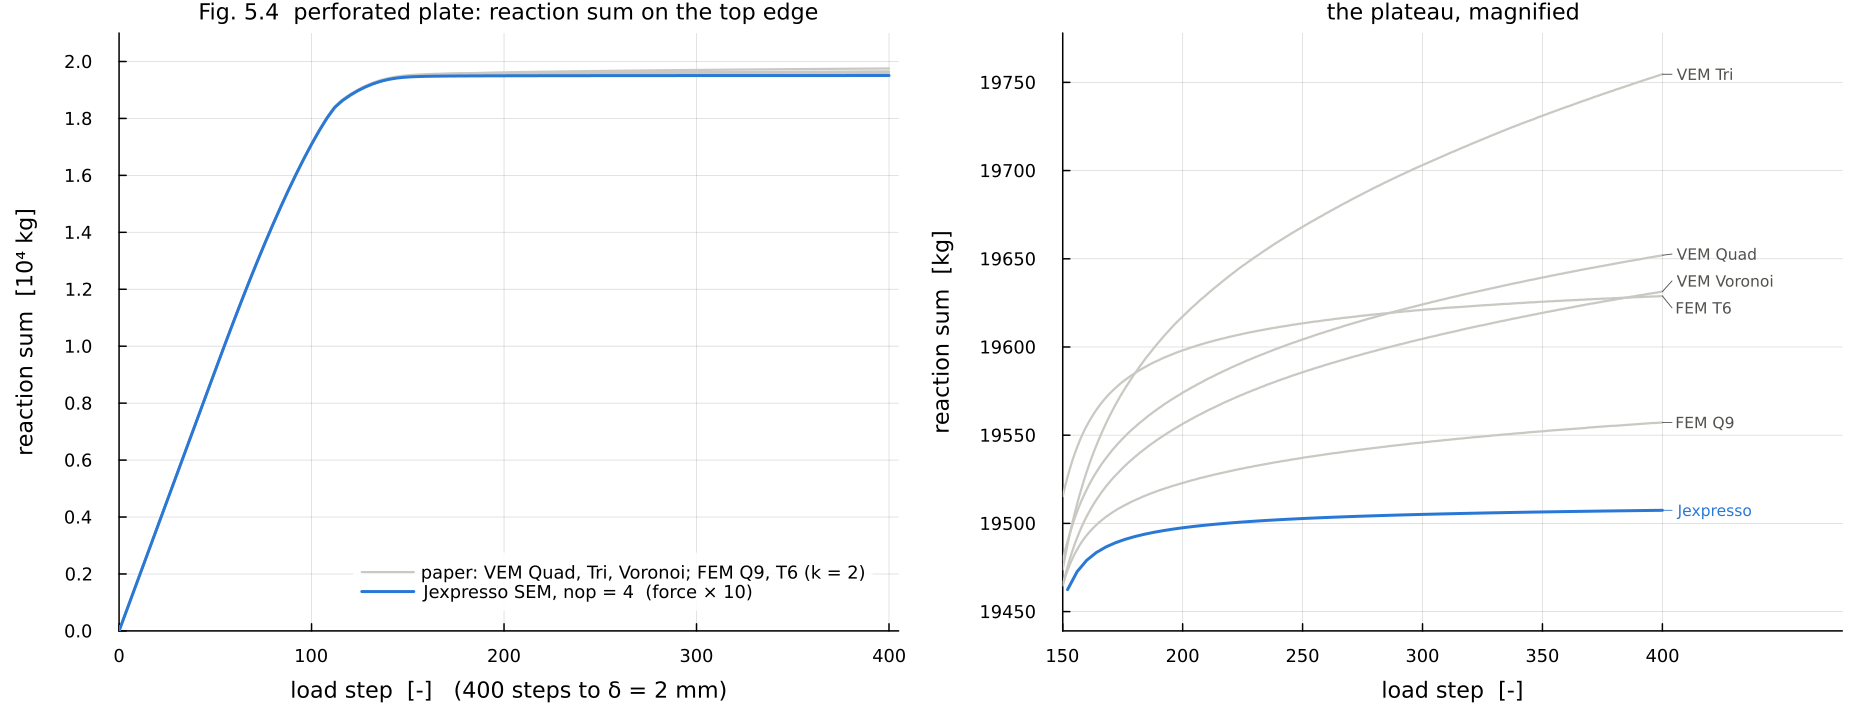
\includegraphics[width=\textwidth]{figures_quasistatic_solid/plate_reaction.png}
\caption{The paper's Fig.~5.4 redrawn by \code{tools/artioli2017\_figures.jl}: the
reaction sum on the top edge against the load step. Grey: the paper's five
quadratic methods, read from the vector graphics of the arXiv PDF. Blue:
Jexpresso, summed from the nodal reaction field \code{ry} of the VTK files,
$\times10$ (the paper's plate is 10~mm thick). Right: the plateau, magnified.}
\label{fig:platereaction}
\end{figure}

\begin{figure}[ht]
\centering
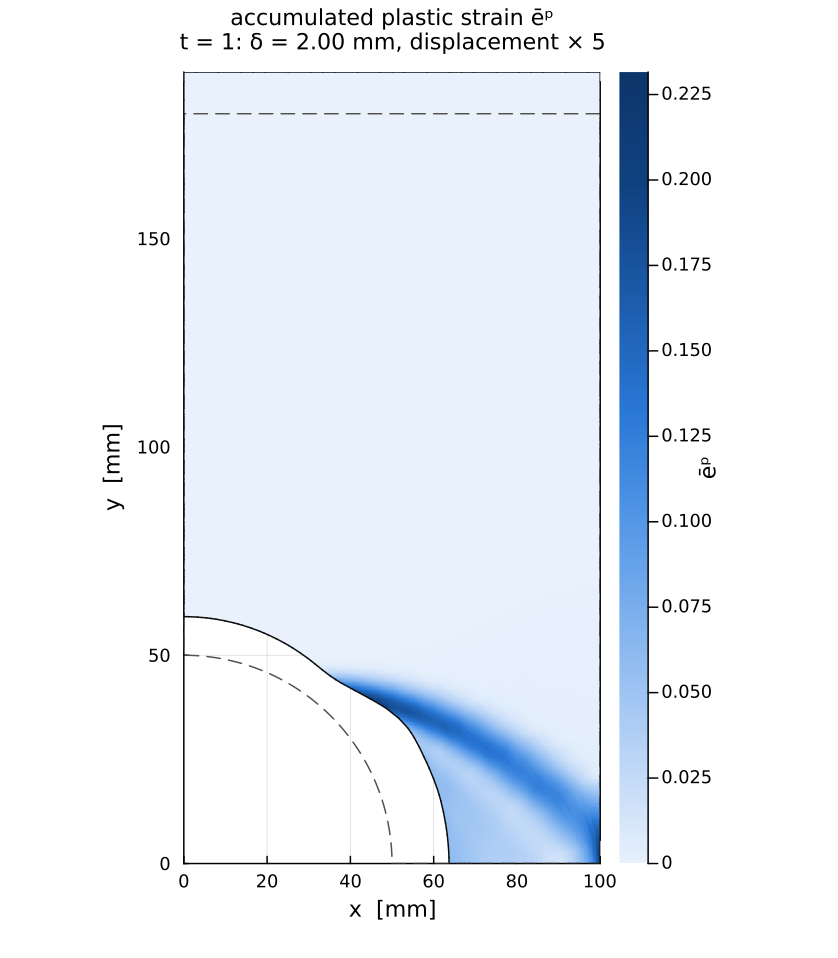
\includegraphics[width=0.48\textwidth]{figures_quasistatic_solid/plate_plastic_strain.png}
\caption{The quarter plate at the end of the loading, displacement $\times5$,
coloured by the accumulated plastic strain $\bar e^p$ (a quadrature-point
history value projected onto the nodes), over the undeformed outline (dashed):
the ligament between the hole and the lateral edge has yielded through, and $A$
has moved towards the lateral edge as the ligament thins.}
\label{fig:platezone}
\end{figure}

\paragraph{Redrawing the paper's figures.} \code{tools/artioli2017\_figures.jl}
runs the three computations at the paper's settings (the viscoelastic cylinder
with both Prony sets and FEAP's load convention, and the plate), reads every
\code{iter\_<k>.pvtu} listed in \code{simulation.pvd} with
\code{tools/vtu\_reader.jl} --- points, fields and cells --- and writes
Fig.~5.2(a,b), Fig.~5.4, Table~1 with Table~2, the plastic zone, and an
animation of the plate deforming beside its reaction curve:
\begin{verbatim}
julia --project=. tools/artioli2017_figures.jl            # run, then plot
julia --project=. tools/artioli2017_figures.jl --no-run   # replot earlier runs
\end{verbatim}
\coderef{\jx{tools/artioli2017_figures.jl}{272}{figure\_5\_4},
the force scale \jx{tools/artioli2017_figures.jl}{245}{PAPER\_FORCE\_SCALE};
the reader \jx{tools/vtu_reader.jl}{203}{read\_vtu};
the test \jxfile{test/test_perforated_plate.jl}{test/test\_perforated\_plate.jl}.}

\section*{References}
\begin{itemize}[nosep,leftmargin=*]
\item E.~Artioli, L.~Beir\~ao da Veiga, C.~Lovadina, E.~Sacco, \emph{Arbitrary order 2D virtual
  elements for polygonal meshes: Part II, inelastic problem}, Comput.\ Mech.\ 60 (2017)
  643--657, \href{https://arxiv.org/abs/1701.06676}{arXiv:1701.06676}.
\item J.~C.~Simo, T.~J.~R.~Hughes, \emph{Computational Inelasticity}, Springer (1998), \S3.3, \S10.3.
\item O.~C.~Zienkiewicz, R.~L.~Taylor, D.~D.~Fox, \emph{The Finite Element Method for Solid and
  Structural Mechanics}, 7th ed., Butterworth--Heinemann (2014).
\item R.~Hill, \emph{The Mathematical Theory of Plasticity}, Oxford (1950).
\item D.~A.~Kopriva, \emph{Metric identities and the discontinuous spectral element method on
  curvilinear meshes}, J.\ Sci.\ Comput.\ 26 (2006) 301--327.
\end{itemize}

\end{document}
